\chapter{Differentialformen auf Mannigfaltigkeiten}
\label{\detokenize{manifolds/manifolds:differentialformen-auf-mannigfaltigkeiten}}\label{\detokenize{manifolds/manifolds::doc}}
\par
In diesem Kapitel der Vektoranalysis werden wir nun \href{https://de.wikipedia.org/wiki/Differentialform}{Differentialformen} einführen.
Die entscheidende Neuerung im Vergleich zum vorangegangen Kapitel über Tensoren ist, dass wir zusätzlich zur Vektorraumstruktur nun ein Konzept von Räumlichkeit einführen.

\par
Außerdem werden wir im Folgenden mit \emph{glatten Funktion} arbeiten, d.h., mit Funktionen aus dem Raum \(C^\infty(U,\R^n)\).
Wir definieren zunächst den Begriff des topologischen Raums als Verallgemeinerung von metrischen Vektorräumen.
Anschließend sind wir in der Lage Mannigfaltigkeiten als spezielle topologische Räume zu definieren, die lokal dem Euklidischen Raum \(\R^n\) ähneln, jedoch global verschieden sein können.
Schließlich werden wir Tensorfelder und Differentialformen diskutieren.


\section{Differenzierbare Mannigfaltigkeit}
\label{\detokenize{manifolds/manifolds_prelim:differenzierbare-mannigfaltigkeit}}\label{\detokenize{manifolds/manifolds_prelim::doc}}

\subsection{Topologische Räume}
\label{\detokenize{manifolds/manifolds_prelim:topologische-raume}}
\par
Wir haben bisher immer Mathematik auf \textbf{metrischen} oder gar \textbf{normierten Vektorräumen} betrieben, da uns diese Struktur für alle erklärten Konzepte am dienlichsten war (siehe Kapitel 4 \& 5 in \cite{Bur20} und \href{https://fau-ammn.github.io/MathDataScience2/normierte\_raeume/normierte\_raeume.html}{MP 2 Skript}).
Als Vorbereitung für \cref{manifolds/manifolds_prelim:s-mannigfaltigkeiten}  wollen wir von den metrischen Räumen zu allgemeineren Strukturen wechseln   den sogenannten \textbf{topologischen Räumen}.

\par
Das zentrale Konzept topologischer Räume ist die folgende Definition der \emph{offene Mengen}.
\begin{definition}{(Offene Mengen und topologischer Raum)}{manifolds/manifolds_prelim:definition-0}



\par
Sei \(\M\) eine Menge und \(\tau \subset \mathcal{P}(M)\) eine Teilmenge der Potenzmenge.
Wir nennen das Tupel \((\M,\tau)\) \textbf{topologischer Raum}, falls die folgenden Eigenschaften erfüllt sind,
\begin{itemize}
\item {} 
\par
\(\emptyset, \M \in \tau\),

\item {} 
\par
für eine beliebige (insbesondere auch \emph{unendlich große}) Indexmenge \(\mathcal{I}\) seien \(U_i\in\tau, i\in \mathcal{I}\). Dann gilt auch schon \(\bigcup_{i\in I} U_i \in \tau\),

\item {} 
\par
für \emph{endlich viele} \(U_j\in\tau, j=1,\ldots, k\) gilt auch schon \(\bigcap_{j=1}^k U_j \in \tau\).

\end{itemize}

\par
Wir bezeichnen mit \(\tau\) die \textbf{Topologie} des Raumes und dessen Elemente \(U\in\tau\) heißen \textbf{offene Mengen}.
Für jeden Punkt \(x\in \M\) nennen wir eine offene Menge \(U(x) \in \tau\) \textbf{Nachbarschaft} oder \textbf{Umgebung} um \(x\), falls \(x\in U(x)\).

\par
Analog zur Definition auf metrischen Räumen bezeichnen wir das Komplement \(\M \setminus U\) \textbackslash{}einer offenen Menge \(U\) als \textbf{abgeschlossen}.
\end{definition}

\par
Es gibt viele interessante topologische Räume, die den Namen ihrer Entdecker tragen, wie zum Beispiel der \href{https://de.wikipedia.org/wiki/Arens-Fort-Raum}{Arens Fort Raum}, der \href{https://de.wikipedia.org/wiki/Cantor-Raum}{Cantor Raum}, oder der \href{https://de.wikipedia.org/wiki/Hilbertw\%C3\%BCrfel}{Hilbertwürfel}.
Im Folgenden wollen wir ein relativ generisches Beispiel für einen topologischen Raum betrachten.
\begin{example}{(Diskrete Topologie)}{manifolds/manifolds_prelim:ex:diskreteTopologie}



\par
Es sei \(M\) eine beliebige Menge.
Dann können wir eine Topologie \(\tau\) auf \(\M\) definieren, in dem wir alle Teilmengen von \(\M\) als offen definieren.
In diesem Beispiel folgt trivialerweise, dass \(\tau = \mathcal{P}(\M)\) gilt.
Dann ist \((\M, \tau)\) ein topologischer Raum.
Diese Topologie nennt man \textbf{diskrete Topologie}, da für jeden diskreten Punkt \(x \in \M\) die Menge \(\lbrace x \rbrace\) offen ist.

\par
Die diskrete Topologie wird durch eine spezielle Metrik erzeugt, wie man im Folgenden einsieht.
Seien \(x,y \in M\) Punkte der Menge und \(d \colon \M \times \M \rightarrow \R^+_0\) eine Metrik auf \(\M\) mit
\begin{align*}
d(x,y) := \begin{cases} 0, \quad \text{ falls } x=y,\\ 1, \quad \text{ falls } x\neq y. \end{cases}
\end{align*}
\par
Über diese Metrik kann man nun \emph{offene Umgebungen} von Punkten \(x \in \M\) wie folgt konstruieren,
\begin{align*}
B_1(x) := \lbrace y \in \M : d(x,y) < 1 \rbrace = \lbrace x \rbrace.
\end{align*}
\par
Dies führt dazu, dass alle Teilmengen, die nur einen Punkt der Menge enthalten, offen sind.
Über beliebige Vereinigung dieser Punktmengen, lassen sich dann alle Teilmengen der Potenzmenge \(\mathcal{P}(\M)\) als offen definieren und man erhält somit die diskrete Topologie.
\end{example}
\begin{remark}{(Notation von topologischen Räumen)}{manifolds/manifolds_prelim:remark-2}



\par
Häufig spielt die konkrete Wahl einer Topologie \(\tau \subset \mathcal{P}(\M)\) keine Rolle für die mathematischen Aussagen, die man treffen möchte.
Da wir jede beliebige Menge \(\M\) mit der diskreten Topologie aus \cref{manifolds/manifolds_prelim:ex:diskreteTopologie} zu einem topologischen Raum \((\M, \tau)\) ausstatten können, wird die Angabe der konkreten Topologie \(\tau\) häufig ausgelassen.
In solchen Fällen identifiziert man den topologischen Raum einfach mit der zu Grunde liegenden Menge \(\M\), d.h., wir nennen \(\M\) einen topologischen Raum, wenn die konkrete Topologie im gewählten Kontext eindeutig ist oder keine Rolle spielt.
\end{remark}

\par
Viele mathematische Konzepte lassen sich von metrischen oder normierten Räumen auf topologische Räume übertragen, wie zum Beispiel der Begriff einer stetigen Funktion.
\begin{definition}{(Stetige Funktionen auf topologischen Räumen)}{manifolds/manifolds_prelim:def:stetigkeitTopologie}



\par
Seien \((\M_1, \tau_1)\) und \((\M_2, \tau_2)\) topologische Räume und \(f\) eine Funktion mit
\begin{align*}
f \colon (\M_1, \tau_1) \rightarrow (\M_2, \tau_2).
\end{align*}
\par
Wir nennen \(f\) \textbf{stetig}, wenn die Urbilder offener Mengen in \(\tau_2\) unter \(f\) wieder offene Mengen in \(\tau_1\) ergeben, d.h.,
\begin{align*}
f \ \text{ stetig } \quad \Leftrightarrow \quad \forall \, O \in \tau_2 : f^{-1}(O) \in \tau_1.
\end{align*}\end{definition}

\par
Das folgende Diagramm zeigt die Relationen zwischen verschiedenen mathematischen Konzepten innerhalb einer hierarchischen Struktur.
\begin{align*}
\begin{gathered}
\text{Skalarprodukt (Euklidischer / Unitärer Vektorraum)}\\
\downarrow \text{induziert}\\
\text{Norm (Normierter Vektorraum)}\\
\downarrow \text{induziert}\\             
\text{Metrik (Metrischer Vektorraum)}\\
\downarrow \text{induziert}\\                 
\text{Topologie (Topologischer Vektorraum)}
\end{gathered}
\end{align*}

\subsection{Mannigfaltigkeiten}
\label{\detokenize{manifolds/manifolds_prelim:mannigfaltigkeiten}}\label{\detokenize{manifolds/manifolds_prelim:s-mannigfaltigkeiten}}
\par
In diesem Abschnitt führen wir das grundlegende Konzept von \href{https://de.wikipedia.org/wiki/Mannigfaltigkeit}{Mannigfaltigkeiten} als Spezialfall eines topologischen Raums ein, der lokal mit dem Euklidischen Raum \(\R^n\) identifiziert werden kann.
Mannigfaltigkeiten spielen insbesondere im mathematischen Teilgebiet der \href{https://de.wikipedia.org/wiki/Differentialgeometrie}{Differentialgeometrie} eine zentrale Rolle.


\subsubsection{Motivation}
\label{\detokenize{manifolds/manifolds_prelim:motivation}}
\par
Das wohl verständlichste Bild einer Mannigfaltigkeit ist die Oberfläche einer dreidimensionalen Kugel
\begin{align*}
\mathbb{S}^2 := \lbrace (x,y,z)\in\R^3 : x^2 + y^2 + z^2 = 1 \rbrace,
\end{align*}
\par
wie sie zum Beispiel genutzt wird um die Erdoberfläche zu modellieren.
Möchte man Mathematik auf solch einer Oberfläche betreiben, so benötigt man vollkommen andere Konzepte als in offenen Teilmengen des \(\R^n\).
Möchte man beispielsweise berechnen, wie weit man reisen muss, um von einem Punkt auf der Oberfläche zu einem anderen Punkt zu kommen, so benötigt man einen angepassten Abstandsbegriff, da die Euklidische Norm nur die direkte Entfernung messen würde, welche die Kugeloberfläche jedoch durchschneidet.
Dies ist in folgender Abbildung visualisiert.

\begin{figure}[htbp]
\centering


\noindent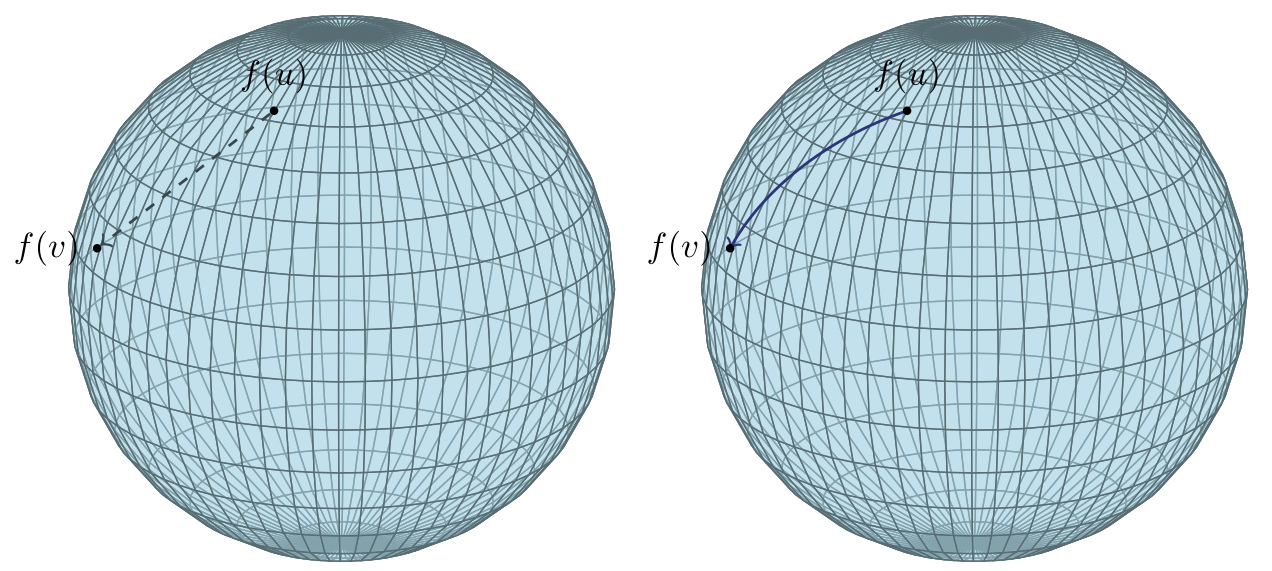
\includegraphics[width=\textwidth]{../\string_build/html/\string_images/mannigfaltigkeit.png}
\caption{Visualisierung zweier unterschiedlicher Abstandsbegriffe für Punkte auf der Kugeloberfläche \(\mathbb{S}^2\).}\label{\detokenize{manifolds/manifolds_prelim:fig-kugel}}\end{figure}

\par
Aus dieser Anschauung wird klar, dass unser bisheriges Konzept von Differenzierbarkeit im Mehrdimensionalen aus dem \href{https://fau-ammn.github.io/MathDataScience2/ableitungen/ableitungen.html}{MP 2 Skript} nicht ausreicht, um auf diesem Objekt geeignet Funktionen abzuleiten.
Da man in vielen Bereichen der Physik und der Mathematik nicht nur auf offenen Teilmengen des \(\R^n\) ableiten möchte, benötigen wir ein analoges Prinzip für topologische Räume \(\M := (\M, \tau)\).

\par
\textbf{Wie können wir den Ableitungsbegriff auf topologische Räume übertragen?}

\par
Die grundlegende Idee ist es, den topologischen Raum \(\M\) lokal mit einer Teilmenge des \(\R^n\) zu identifizieren.
Für eine beliebige offene Teilmenge \(U\subset \M\) betrachten wir also eine Abbildung
\begin{align*}
\phi:U\rightarrow \R^n.
\end{align*}
\par
Wir wollen fordern, dass es sich bei \(\phi\) um eine \emph{injektive Abbildung} handelt, so dass eine inverse Abbildung \(\phi^{-1}\) existiert.
Diese Umkehrabbildung müssen wir jedoch auf das Bild \(\phi(U) \subset \R^n\) einschränken, damit sie wohldefiniert ist.
Damit erhalten wir eine \emph{lokale Bijektion} \(\phi^{-1}:\phi(U)\rightarrow U\).

\par
Betrachten wir nun eine Funktion \(f \colon \M \rightarrow \R^m\), die Punkte des topologischen Raumes auf Punkte des \(\R^m\) abbildet.
Wenn wir diese Funktion differenzieren möchten, so sehen wir ein, dass die Verknüpfung
\begin{align*}
f \circ \phi^{-1} : \phi(U) \subset \R^n \to \R^m
\end{align*}
\par
es uns erlaubt, das Problem der Ableitung in topologischen Räumen auf das Konzept der mehrdimensionalen Differentiation im \(\R^n\) zurückzuführen.


\subsubsection{Karten und Atlanten auf topologischen Räumen}
\label{\detokenize{manifolds/manifolds_prelim:karten-und-atlanten-auf-topologischen-raumen}}
\par
Um den Ableitungsbegriff auf topologischen Räumen \(\M\) formal definieren zu können, benötigen wir zusätzlich zur Bijektivität der Abbildung \(\phi \colon U \rightarrow \phi(U) \subset \R^n\) die Bedingung, dass für jede Teilmenge \(U \subset \M\) gilt,
\begin{align*}
\phi(U)\text{ ist offen} \ \Leftrightarrow \ U \text{ ist offen}.
\end{align*}
\par
Diese Forderung bedeutet, dass offene Teilmengen in \(U \subset \M\) gerade mit offenen Teilmengen in \(\phi(U) \subset \R^n\) identifiziert werden.
Wir wollen im Folgenden beide Implikationsrichtungen diskutieren.

\par
1. \(\phi(U)\) ist offen \(\Rightarrow U \) ist offen.

\par
Diese Implikation ist äquivalent zur Forderung, dass Urbilder offener Mengen selbst wieder offen sind.
Mit \cref{manifolds/manifolds_prelim:def:stetigkeitTopologie} bedeutet dies wiederum, dass die Abbildung \(\phi\) stetig ist.

\par
2. \(\phi(U)\) ist offen \(\Leftarrow U \) ist offen.

\par
Analog zur obigen Überlegung sehen wir ein, dass diese Bedingung gerade aussagt, dass \(\phi^{-1}\) stetig ist.
Diese Forderung ist nicht immer trivialerweise erfüllt.

\par
Das folgende Beispiel zeigt, dass es tatsächlich stetige bijektive Abbildung \(\phi\) gibt, für die gilt, dass die Umkehrabbildung \(\phi^{-1}\) \emph{nicht stetig} ist.
\begin{example}{}{manifolds/manifolds_prelim:ex:nonho}



\par
Wir betrachten in diesem Beispiel die Funktion
\begin{align*}
\phi:[0,2\pi)&\to\R^2,\\
t &\mapsto \phi(t):= (\cos(t), \sin(t)).
\end{align*}
\par
Wir erkennen, dass \(\phi([0,2\pi)) = \S^1\) gerade der Einheitskreis ist, und dass \(\phi:[0,2\pi)\to\S^1\) bijektiv und stetig ist.
Allerdings stellen wir fest, dass die Umkehrabbildung nicht stetig ist.
Sei dazu \((x_i)_{i\in\N}\) eine Folge von Punkten auf dem Einheitskreis \(\S^1\), deren \(y\) Koordinate negativ ist und die gegen den Punkt \(x = (1,0) \in \S^1\) konvergieren, d.h.,
\begin{align*}
\lim_{i\rightarrow\infty} x_i =: x = (1,0) \in \S^1.
\end{align*}
\par
Betrachten wir jedoch den Grenzwert der Folge von Funktionswerten \((\phi^{-1}(x_i))_{i\in I}\), so sehen wir, dass
\begin{align*}
\lim_{i\to\infty} \phi^{-1} (x_i) = 2\pi \neq 0 = \phi^{-1}(x)
\end{align*}
\par
und somit ist \(\phi^{-1}\) offensichtlich nicht stetig.
\end{example}

\begin{figure}[htbp]
\centering


\noindent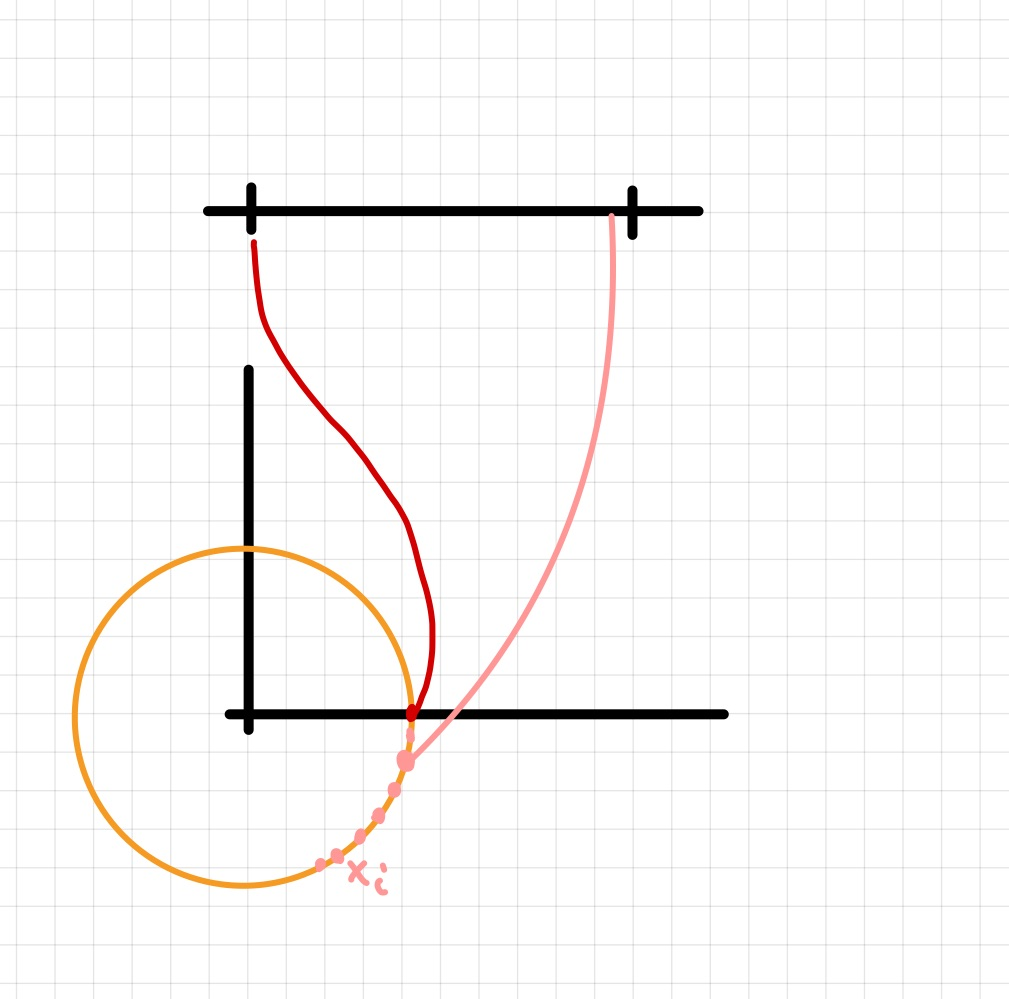
\includegraphics[width=\textwidth]{../\string_build/html/\string_images/nonhomöo.jpg}
\caption{Visualisierung einer unstetigen Umkehrabbildung für das \cref{manifolds/manifolds_prelim:ex:nonho} }\label{\detokenize{manifolds/manifolds_prelim:fig-nonh}}\end{figure}

\par
Insgesamt fordern wir also, dass \(\phi:U\rightarrow\phi(U)\) bijektiv ist und zusätzlich, dass sowohl \(\phi\) als auch die Umkehrabbildung \(\phi^-1\) stetig sind.
Eine solche Abbildung definiert man unter dem Begriff \emph{Homöomorphismus}.
\begin{definition}{(Homöomorphismus)}{manifolds/manifolds_prelim:definition-5}



\par
Seien \(X\) und \(Y\) topologische Räume.
Dann nennen wir eine Abbildung \(f \colon X \rightarrow Y\) einen \textbf{Homöomorphismus}, wenn sie folgende Eigenschaften erfüllt:
\begin{enumerate}

\item {} 
\par
\(f\) ist bijektiv

\item {} 
\par
\(f\) ist stetig

\item {} 
\par
die Umkehrfunktion \(f^{-1}\) ist ebenfalls stetig.

\end{enumerate}
\end{definition}

\par
Speziell im Kontext von Mannigfaltigkeiten \(\M\), als Spezialfall topologischer Räume (wie wir noch sehen werden), nennt man eine offene Menge zusammen mit einem Homöomorphismus eine \textbf{Karte} auf \(\M\).
\begin{definition}{(Karte)}{manifolds/manifolds_prelim:definition-6}



\par
Es sei \(\M\) ein topologischer Raum und \(U\subset\M\) eine offene Menge.
Sei außerdem \(\phi:U\rightarrow \phi(U)\subset \R^n\) ein Homöomorphismus.
Dann heißt das Tupel \((U,\phi)\) \textbf{Karte} auf \(\M\).
\end{definition}

\par
Um einen Ableitungsbegriff für Funktionen \(f:\M\to\R^m\) über eine Karte \((U,\phi)\) und der Verknüpfung \(f\circ \phi^{-1}\) zu definieren benötigen wir noch ein zusätzliches Konzept.
Denn in der Situation, dass \((V,\psi)\) eine zweite Karte ist, deren offene Menge \(V\) einen nichtleeren Schnitt mit der offenen Menge \(U\) hat, d.h., \(U\cap V \neq \emptyset\), erhalten wir genau auf dem Schnitt dieser Mengen zwei unterschiedliche Parametrisierungen,
\begin{align*}
f\circ \phi^{-1} = (f\circ\psi^{-1})\circ(\psi\circ \phi^{-1}),\\
f\circ \psi^{-1} = (f\circ\phi^{-1})\circ(\phi\circ \psi^{-1}).
\end{align*}
\par
Um von einer Karte zur nächsten Karte zu kommen benötigen wir eine geeignete Abbildung.
\begin{definition}{(Kartenwechsel)}{manifolds/manifolds_prelim:definition-7}



\par
Es sei \(\M\) ein topologischer Raum und es seien \((U,\phi)\) und \((V,\psi)\) zwei Karten auf \(\M\) mit nicht leerem Schnitt, d.h., \(U\cap V\neq \emptyset\).
Dann nennt man die Abbildung
\begin{align*}
\psi\circ\phi^{-1}: \phi(U\cap V)\rightarrow \psi(U\cap V)
\end{align*}
\par
einen \textbf{Kartenwechsel} von \((U,\phi)\) nach \((V,\psi)\).
\end{definition}

\begin{figure}[htbp]
\centering


\noindent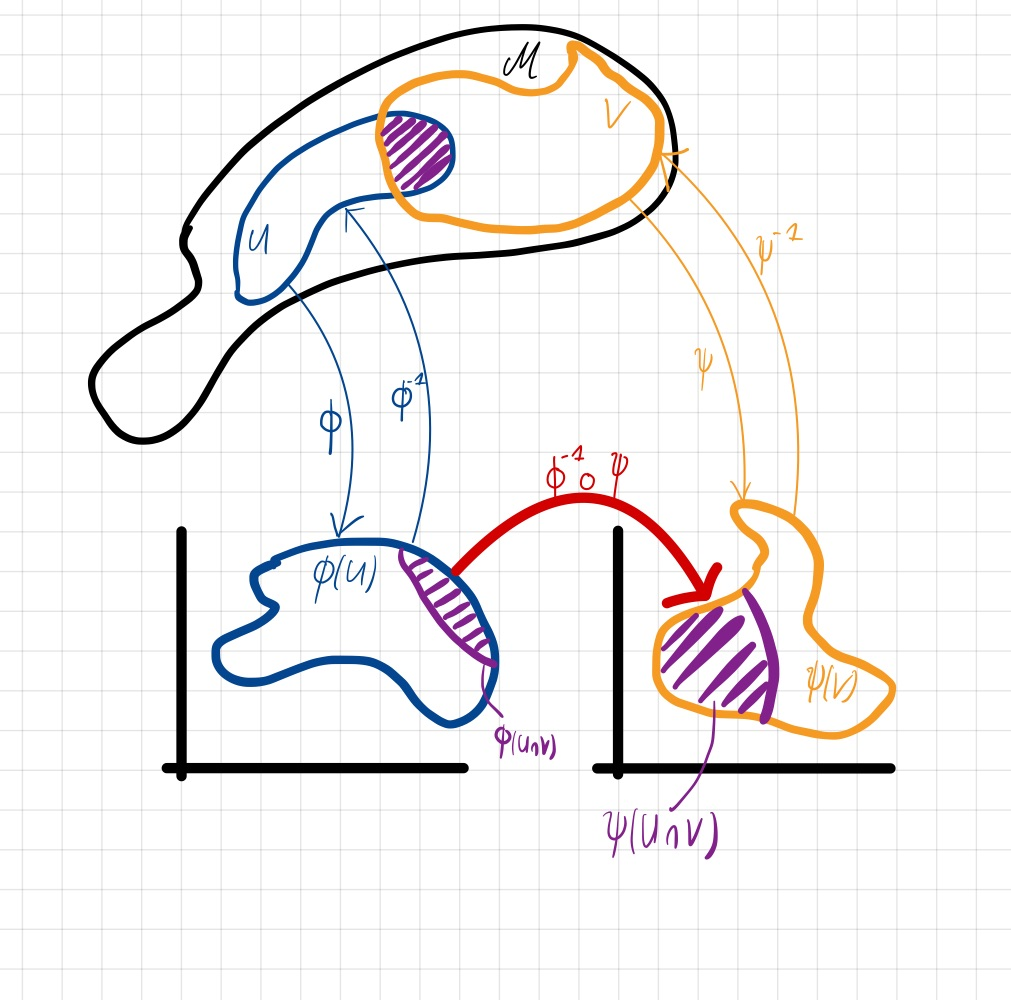
\includegraphics[width=\textwidth]{../\string_build/html/\string_images/chartchange.jpg}
\caption{Kartenwechsel.}\label{\detokenize{manifolds/manifolds_prelim:fig-chartchange}}\end{figure}

\par
Wir erkennen also, dass Umparametrisierungen der Form \(\psi\circ \phi^{-1}\) entscheidend sind, um von einer lokalen Identifikation des topologischen Raums zur nächsten zu gelangen.
Wäre nun der Kartenwechsel \(\psi\circ \phi^{-1}\) und respektive \(\phi\circ \psi^{-1}\) differenzierbar, so könnte man die jeweiligen Ableitungen leicht durch die Kettenregel ineinander umrechnen.
Allerdings existieren durchaus Beispiele, in denen sowohl \(f\circ\phi^{-1}\) als auch \(f\circ\psi^{-1}\) differenzierbar sind, aber der Kartenwechsel \(\psi\circ\phi^{-1}\) nicht.
Deshalb führt man zusätzlich noch den folgenden Begriff ein.
\begin{definition}{(Atlas)}{manifolds/manifolds_prelim:definition-8}



\par
Es sei \(\M\) ein topologischer Raum.
Eine Familie von Karten \(\mathcal{A} = (U_i,\phi_i)_{i\in I}\) indiziert durch die Indexmenge \(I\) heißt \textbf{Atlas}, falls die Vereinigung aller offenen Mengen eine Überdeckung des topologischen Raums darstellt, d.h., es gilt
\begin{align*}
\M = \bigcup_{i\in I} U_i.
\end{align*}
\par
Wir nennen einen Atlas \(k\) mal \textbf{differenzierbar} oder von der Klasse \(C^k\), falls jeder Kartenwechsel \(\phi_i\circ\phi_j^{-1}, i,j\in I\) \(k\) mal stetig differenzierbar ist.
\end{definition}

\par
Die Begriffe \emph{Karte} und \emph{Atlas} stammen in der Tat aus mathematischen Überlegungen in der Kartographie.
Man kann Teile der Erdoberfläche mit einer Karte auf eine Ebene \(\R^2\) abbilden.
Nähert man sich dem Rand einer Karte, so möchte man zu einer anderen Karte wechseln, die das angrenzende Gebiet darstellt.

\par
So kann eine Mannigfaltigkeit durch einen vollständigen Satz von Karten vollständig beschrieben werden; man braucht dabei Regeln, wie sich beim Kartenwechsel die Karten überlappen.


\subsubsection{Differenzierbare Mannigfaltigkeiten}
\label{\detokenize{manifolds/manifolds_prelim:differenzierbare-mannigfaltigkeiten}}
\par
Für einen topologischen Raum \(\M\) können mehrere Atlanten \(\mathcal{A}\) existieren, weshalb es sinnvoll ist Äquivalenzklassen von Atlanten zu betrachten.
\begin{definition}{(\protect\(C^k\protect\) differenzierbare Struktur)}{manifolds/manifolds_prelim:definition-9}



\par
Für einen Index \(k\in \N \cup \{\infty\}\) heißen zwei differenzierbare Atlanten \(\mathcal{A}_1, \mathcal{A}_2\) der Klasse \(C^k\) \textbf{\(k\) äquivalent}, falls ihre Vereinigung \(\mathcal{A}_1\cup \mathcal{A}_2\) wieder ein Atlas der Klasse \(C^k\) ist.
Dies bedeutet insbesondere, dass die Kartenwechsel durch die Vereinigung der beiden Atlanten weiterhin \(k\) mal stetig differenzierbar bleiben.
In diesem Fall notieren wir \(\mathcal{A}_1\sim_k \mathcal{A}_2\).
Die Äquivalenzklasse \([\mathcal{A}]_{\sim_k}\) nennt man eine \textbf{\(C^k\) differenzierbare Struktur}.
\end{definition}

\begin{emphBox}{}{}

\par
\href{https://de.wikipedia.org/wiki/Felix\_Hausdorff}{Felix Hausdorff} (geboren am 8. November 1868 in Breslau; gestorben am 26. Januar 1942 in Bonn) war ein deutscher Mathematiker.
\end{emphBox}

\par
Bisher haben wir \(\M\) als allgemeinen topologischen Raum betrachtet.
In vielen Anwendungen benötigt man aber weitere nützliche Eigenschaften des Raumes.
Insbesondere wenn man \href{https://de.wikipedia.org/wiki/Testfunktion}{glatte Testfunktionen} und \href{https://en.wikipedia.org/wiki/Partition\_of\_unity}{die Zerlegung der Eins} benutzen möchte braucht man folgende zwei zusätzliche Eigenschaften.

\par
Wir definieren zunächst die Eigenschaft eines Hausdorff Raums.
\begin{definition}{(Hausdorff Raum)}{manifolds/manifolds_prelim:def:hausdorffraum}



\par
Ein topologischer Raum \(\M\) heißt \textbf{Hausdorff Raum}, falls für je zwei unterschiedliche Punkte \(x,y\in \M, x\neq y\) offene Umgebungen \(U(x), U(y) \subset \M\) existieren, welche disjunkt sind, d.h., \(U(x)\cap U(y) = \emptyset\).
Man nennt \(\M\) dann auch einen \textbf{separierten Raum}.
\end{definition}

\par
Als zweite nützliche Eigenschaft fordern wir, dass unser topologischer Raum \(\M\) das zweite Abzählbarkeitsaxiom erfüllen soll.
\begin{definition}{(Zweites Abzählbarkeitsaxiom)}{manifolds/manifolds_prelim:definition-11}



\par
Ein toplogischer Raum \((\M, \tau)\) erfüllt das \textbf{zweite Abzählbarkeitsaxiom}, falls \emph{abzählbar} viele offene Mengen \((V_i)_{i\in\N} \in \tau\) existieren, so dass für jeden Punkt \(x\in \M\) und jede offene Umgebung \(U(x) \in \tau\) von \(x\) mindestens ein Index \(k\in\N\) existiert mit \(V_k \subset U(x)\).
Man nennt \((\M, \tau)\) dann auch \textbf{zweitabzählbar}.
\end{definition}

\par
Diese zwei Bedingung wirken zunächst abstrakt.
Glücklicherweise werden sie jedoch von vielen üblichen topologischen Räumen erfüllt, wie zum Beispiel dem Euklidischen Raum \(\R^n\).
\begin{remark}{}{manifolds/manifolds_prelim:remark-12}



\par
Falls der Begriff eines zweitabzählbaren Hausdorff Raums zu unhandlich erscheint, kann man für die meisten Anwendungen in der Physik auch einfach \textbf{metrische Räume} betrachten, die diese beiden Eigenschaften implizieren.
\end{remark}

\par
Nun haben wir alle nötigen Voraussetzungen geschaffen um den Begriff einer Mannigfaltigkeit formal einzuführen.
\begin{definition}{}{manifolds/manifolds_prelim:definition-13}



\par
Es sei \(\M\) ein zweitabzählbarer Hausdorff Raum und für \(k\in\N\cup \{\infty\}\) sei \([\mathcal{A}]_{\sim_k}\) eine \(C^k\) differenzierbare Struktur.
Dann nennen wir \((\M,[\mathcal{A}]_{\sim_k})\) eine \(k\) \textbf{mal differenzierbare Mannigfaltigkeit}.
Für den Spezialfall \(k=\infty\) sprechen wir auch von einer \textbf{glatten Mannigfaltigkeit}.

\par
Falls alle Karten auf \(\M\) nach \(\R^n\) abbilden, so nennt man die Mannigfaltigkeit \emph{\(n\) dimensional}.
\end{definition}

\par
Ähnlich wie bei topologischen Räumen spricht man in den meisten Fällen nur von der Mannigfaltigkeit \(\M\); die differenzierbare Struktur \([\mathcal{A}]_{\sim_k}\) wird dabei implizit vorausgesetzt.

\par
Basierend auf einer differenzierbaren Mannigfaltigkeit \(\M\) können wir nun differenzierbare Funktionen auf \(\M\) definieren.
\begin{definition}{}{manifolds/manifolds_prelim:definition-14}



\par
Sei \(\M\) eine \(k\) mal differenzierbare Mannigfaltigkeit \(\mathcal{A}\) ein Atlas auf \(\M\).
Dann nennen wir eine Abbildung \(f:\M\to\R^m\) \textbf{\(k\) mal differenzierbar}, falls für jeden Punkt \(x\in\M\) eine differenzierbare Karte \((U(x),\phi)\in\mathcal{A}\) existiert, so dass \(f\circ\phi^{-1} \in C^k(\phi(U(x)); \R^m)\).
Insbesondere schreiben wir in diesem Fall \(f\in C^k(\M; \R^m)\).
\end{definition}

\par
In vielen Anwendungen beschränkt man sich nur auf \emph{glatte Mannigfaltigkeiten} und \emph{glatte Funktionen} in \(C^\infty(\M; \R^m)\).
Wir werden im Folgenden der Einfachheit halber auch dazu übergehen.
\begin{lemma}{}{manifolds/manifolds_prelim:lemma-15}



\par
Es sei \(\M\) eine glatte Mannigfaltigkeit.
Dann ist \(C^\infty(\M; \R^m)\) ein reeller Vektorraum mit den Verknüpfungen
\begin{align*}
(\lambda \cdot f)(x) := \lambda\cdot f(x)\text{ für } f\in C^\infty(\M; \R^m), \lambda\in\R,\\
(f + g)(x) := f(x) + g(x)\quad\text{ für } f,g\in C^\infty(\M; \R^m).
\end{align*}\end{lemma}

\begin{proof}
 In der Hausaufgabe zu zeigen.
\end{proof}

\par
Die Eigenschaft der Differenzierbarkeit einer Funktion auf einer Mannigfaltigkeit ist kartenunabhängig, wie folgendes Lemma feststellt.
\begin{lemma}{}{manifolds/manifolds_prelim:lem:differenzierbarkeitKartenunabhaengig}



\par
Es sei \(\M\) eine glatte Mannigfaltigkeit und \(\mathcal{A}\) ein Atlas auf \(\M\).
Außerdem sei \(f:\M \to \R^m\) eine Funktion, \((U,\phi)\in \mathcal{A}\) eine Karte und \(x \in U\) ein Punkt in der offenen Menge \(U\).
Ist \(f\circ\phi^{-1}\) differenzierbar in \(x\), so ist \(f\circ\psi^{-1}\) auch differenzierbar in \(x\) für jede Karte \((V,\psi) \in \mathcal{A}\) mit \(x\in V\).
\end{lemma}

\begin{proof}
 In der Hausaufgabe zu zeigen.
\end{proof}


\section{Tangentialräume und Tangentialbündel}
\label{\detokenize{manifolds/tangential:tangentialraume-und-tangentialbundel}}\label{\detokenize{manifolds/tangential::doc}}

\subsection{Tangentialräume an Mannigfaltigkeiten}
\label{\detokenize{manifolds/tangential:tangentialraume-an-mannigfaltigkeiten}}
\par
Aus dem Kapitel \cref{odestability/ruhelagen:s-linearisierung-ruhelage}  ist bereits das Konzept der \emph{Linearisierung} bekannt.
Anschaulich gesprochen haben wir eine differenzierbare Funktion \(f\) durch ihre Linearisierung ersetzt um ein einfacheres Problem zu erhalten.
Dieses Konzept soll nun auf glatte Mannigfaltigkeiten übertragen werden.

\par
Wir haben bereits erkannt, wie wir den Begriff der Differenzierbarkeit einer Funktion auf einer Mannigfaltigkeit definieren.
Und obwohl die Frage nach der Differenzierbarkeit einer Funktion nach \cref{manifolds/manifolds_prelim:lem:differenzierbarkeitKartenunabhaengig} kartenunabhängig ist, so stellt sich heraus, dass der tatsächliche \emph{Wert der Ableitung} einer Verknüpfung \(f \circ\phi^{-1}\) noch immer von der konkreten Wahl des Homöomorphismus \(\phi\) abhängt.
Um auch hier die gewünschte Kartenunabhängigkeit zu erreichen, brauchen wir einen anderen Begriff der Differenzierbarkeit.
Hierbei wird uns der sogenannte \textbf{Tangentialraum} helfen.
Man kann ihn als eine Linearisierung der Mannigfaltigkeit \(\M\) an einem Punkt \(p\in\M\) interpretieren.

\par
Das folgende Beispiel erklärt anschaulich den Tangentialraum an eine Mannigfaltigkeit.
\begin{example}{}{manifolds/tangential:example-0}



\par
Wir betrachten zunächst den Einheitskreis \(\M = \mathbb{S}^1\) und den Punkt \(p = (1, 0)^T \in \mathbb{S}^1\).
Der Tangentialraum \(T_p\M\) an \(\M\) im Punkt \(p\) ist der eindimensionale Unterraum
\begin{align*}
T_p\M = \lbrace \lambda \cdot (0, 1)^T : \lambda \in \R \rbrace \subset \R^2.
\end{align*}\end{example}

\par
Es gibt in der Literatur zwei verschiedene, jedoch äquivalente Arten den Tangentialraum zu definieren.
\begin{itemize}
\item {} 
\par
\textbf{Geometrischer Tangentialraum}: Bei diesem Ansatz wählt man eine geometrisch Anschauung und definiert den Tangentialraum durch Richtungsvektoren, die am Punkt \(p\in\M\) anliegen.
Der Vorteil dieser Definition ist es, dass sie intuitiv und geometrisch anschaulich ist.

\item {} 
\par
\textbf{Algebraische Defnition}: Bei diesem Ansatz führt man den Tangentialraum mittels spezieller linearer Abbildungen, genannt Derivationen, zurück.
Man verliert hierbei zwar die geometrische Anschauung, allerdings ist das Konzept relativ einfach zu formulieren und hilft die Sachverhalte auf algebraische Zusammenhänge zurückzuführen.

\end{itemize}

\par
In der Praxis (und in vielen Mathematikbüchern) werden beide Definitionen nebeneinander verwendet und die jeweilige Interpretation geht dann aus dem Kontext hervor.
Da sich die beiden Konzepte somit schlecht voneinander trennen lassen werden wir im Folgenden den geometrischen Tangentialraum \(T^{\text{geo}}_p\M\) und den algebraischen Tangentialraum \(T^{\text{alg}}_p\M\) explizit einführen und anschließend eine Isomorphie
\begin{align*}
T^{\text{geo}}_p\M\cong T^{\text{alg}}_p\M
\end{align*}
\par
zwischen den beiden Tangentialräumen zeigen.

\begin{emphBox}{}{}
\par
In der Literatur wird diese explizite Unterscheidung oft nicht vorgenommen.
Stattdessen wird der Tangentialraum einfach nur \(T_p\M\) genannt.
Elemente dieses Raums sind dann je nach Kontext geometrisch oder algebraisch zu interpretieren.
\end{emphBox}


\subsubsection{Geometrische Definition}
\label{\detokenize{manifolds/tangential:geometrische-definition}}
\par
Von der Differentiation im Mehrdimensionalen ist bereits das Konzept der \textbf{Richtungsableitung} bekannt (siehe Kapitel 6.2.2 in \cite{Ten21}).
Hierbei betrachtet man für eine Funktion \(F:\R^n\to\R\) den Strahl \(\gamma(t):= x + t\cdot v\), wobei \(x,v\in\R^n\) und den Grenzwert
\begin{align*}
\lim_{t\to 0} \frac{F(\gamma(t)) - F(\gamma(0))}{t} = \frac{F(x + t\cdot v) - F(x))}{t}.
\end{align*}
\par
Wir werden dieses Konzept nun auf glatte \(n\) dimensionale Mannigfaltigkeiten \(\M\) verallgemeinern, indem wir anstatt von Strahlen differenzierbare \emph{Kurven} auf der Mannigfaltigkeit betrachten.
\begin{definition}{}{manifolds/tangential:definition-1}



\par
Sei \(\M\) eine glatte Mannigfaltigkeit und sei
\begin{align*}
\gamma \colon (-1,1) \rightarrow \M
\end{align*}
\par
eine Kurve auf der Mannigfaltigkeit \(\M\).
Wir nennen \(\gamma\) \textbf{differenzierbar} im Punkt \(0\in(-1,1)\), falls die Kurve \emph{stetig} ist und falls eine Karte \((U,\phi)\) von \(\M\) existiert, so dass für genügend kleines \(\varepsilon\) auch \(\gamma((-\varepsilon,\varepsilon))\subset U\) gilt und die Verknüpfung
\begin{align*}
\phi \circ \gamma:(-\varepsilon,\varepsilon)\to\R^n
\end{align*}
\par
differenzierbar in \(0\) ist .
\end{definition}

\par
Wir werden im Folgenden ausschließlich die Ableitung der Kurve im Punkt \(t=0\) betrachten und sprechen deshalb verkürzt einfach nur von \emph{differenzierbaren} Kurven.
Zusätzlich sei zu bemerken, dass die obige Definition \textbf{nicht} von der Wahl der Karte abhängt.
\begin{example}{}{manifolds/tangential:example-2}



\par
Es sei \(\M=\S^2\) die Einheitssphäre und \(f:\M\to\R\) beschreibe eine Wärmeverteilung auf deren Oberfläche.
Betrachtet man nun die Bahn eines Partikels auf der Oberfläche beschrieben durch die Kurve \(\gamma:(-t, t)\to \M\) so erhalten wir eine eindimensionale Abbildung
\begin{align*}
f\circ\gamma:(-t,t)\to \R,
\end{align*}
\par
die zu jedem Zeitpunkt die Temperatur des Ortes, an dem sich der Partikel befindet, beschreibt.
\end{example}

\begin{figure}[htbp]
\centering


\noindent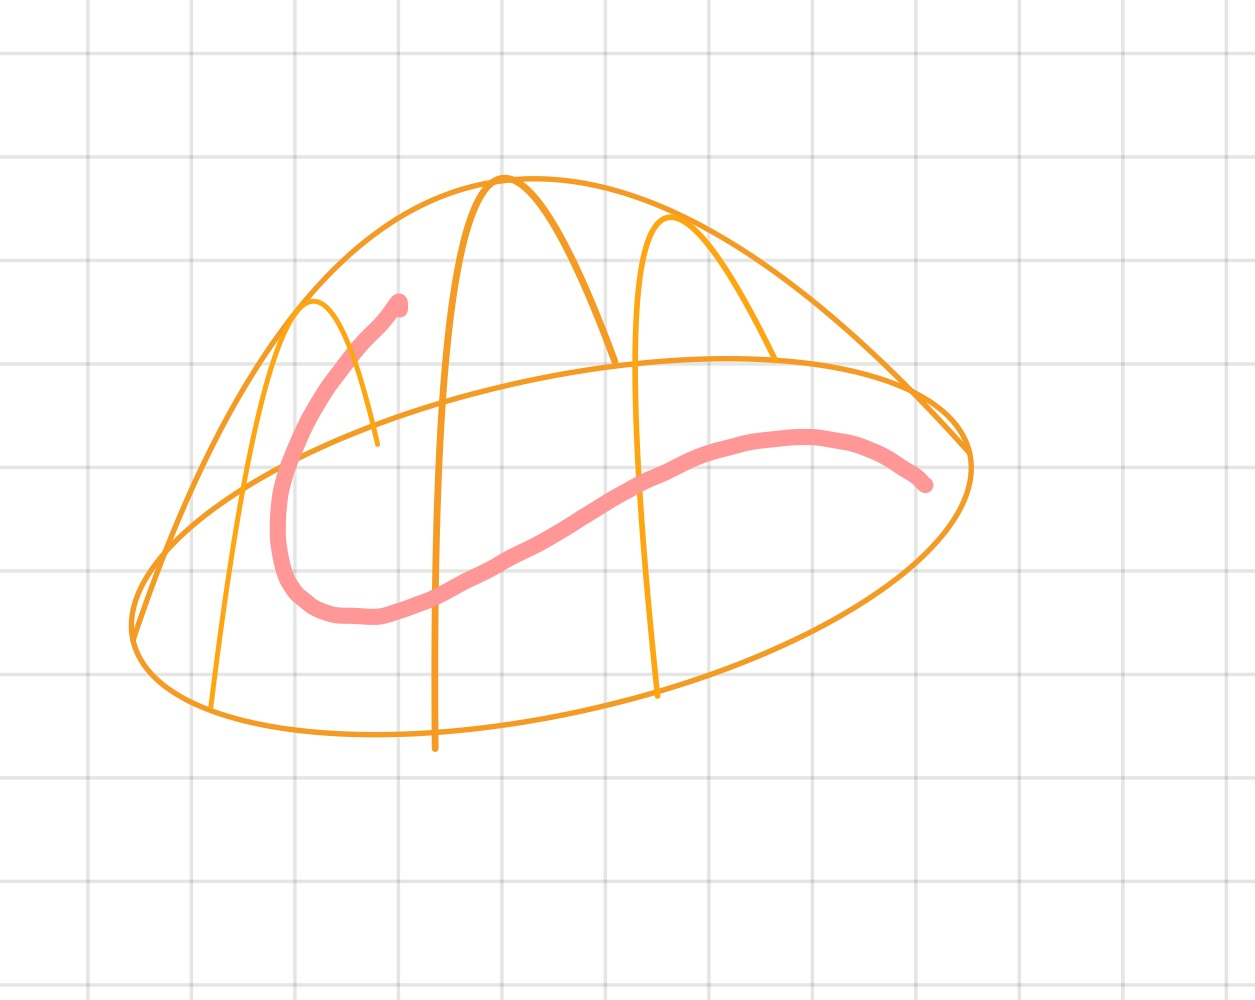
\includegraphics[width=\textwidth]{../\string_build/html/\string_images/velocity.jpg}
\caption{Visualisierung einer Kurve auf der oberen Hälfte der Einheitssphäre im \(\R^3\).}\label{\detokenize{manifolds/tangential:fig-velocity}}\end{figure}

\par
Mit Hilfe von differenzierbaren Kurven auf Mannigfaltigkeiten können wir im Folgenden die Richtungsableitung an einer Mannigfaltigkeit definieren.
\begin{definition}{}{manifolds/tangential:def:direcdiv}



\par
Es sei \(\M\) eine glatte Mannigfaltigkeit, \(\gamma:(-1,1)\to\M\) eine differenzierbare Kurve mit \(\gamma(0)=p\in\M\) und \(f \in C^\infty(\M)\) eine glatte Funktion.
Dann nennen wir die Abbildung
\begin{align*}
D_\gamma : C^\infty(\M) &\to \R\\
f &\mapsto D_\gamma(f):=\frac{d}{dt}(f\circ \gamma)\big\rvert_{t=0}
\end{align*}
\par
\textbf{Richtungsableitung} von \(f\) durch \(\gamma\) im Punkt \(p\).
\end{definition}

\par
Betrachten wir nun eine differenzierbare Kurve \(\gamma \colon (-1, 1) \rightarrow \M\) mit \(\gamma(0)=p \in \M\) und eine glatte Funktion \(f \in \C^\infty(\M)\) definiert auf einer glatten Mannigfaltigkeit \(\M\).
Dann können wir die Richtungsableitung \(D_\gamma(f)\) mit Hilfe der \textbf{Kettenregel für die Differentiation} darstellen als
\begin{align*}
D_\gamma(f) = \frac{d}{dt}(f\circ \gamma)\big\rvert_{t=0} = \frac{d}{dt}\big( (f\circ \phi^{-1}) (\phi \circ \gamma) \big)\rvert_{t=0} = 
\big(D(f\circ \phi^{-1})\big)(\phi(p))\cdot \frac{d}{dt}(\phi \circ \gamma)\rvert_{t=0}
\end{align*}
\par
und für eine weitere differenzierbare Kurve \(\eta \colon (-1, 1) \rightarrow \M\) mit \(\eta(0)=p\) erhalten wir analog
\begin{align*}
D_\eta(f) = \frac{d}{dt}(f\circ \eta)\big\rvert_{t=0} = 
\big(D(f\circ \phi^{-1})\big)(\phi(p))\cdot \frac{d}{dt}(\phi \circ \eta)\rvert_{t=0}.
\end{align*}
\par
Wir erkennen also, dass der Wert der Richtungsableitung in der Tat von der Kurve \(\gamma\) abhängt.
Dies führt auf einen natürlichen Äquivalenzbegriff von Kurven, wie die folgende Bemerkung beschreibt.
\begin{remark}{(Tangentialvektoren)}{manifolds/tangential:rem:tang}



\par
Es sei \(\M\) eine glatte \(n\) dimensionale Mannigfaltigkeit, \(p\in\M\) ein Punkt auf der Mannigfaltigkeit und \((U,\phi)\) eine Karte von \(\M\), für die gilt, dass \(p\in U\) ist.
Für zwei differenzierbare Kurven \(\gamma, \eta:(-1,1) \to U\) mit \(\gamma(0) = \eta(0) = p\) ist die Relation
\begin{align*}
\gamma \sim_p \eta
\qquad \Leftrightarrow \qquad
\frac{d}{dt}(\phi \circ \gamma)\rvert_{t=0} = \frac{d}{dt}(\phi \circ \eta)\rvert_{t=0}\in \R^n
\end{align*}
\par
eine Äquivalenzrelation (siehe Kapitel 2.1.1 in \cite{Bur20}).
Insbesondere ist die Äquivalenzklasse unabhängig von der Wahl des Homöomorphismus \(\phi\).
\end{remark}

\par
Mittels der oben beschriebenen Äquivalenzrelation sind wir in der Lage den Begriff der \emph{Tangentialvektoren} und des \emph{Tangentialraums} zu definieren.
\begin{definition}{}{manifolds/tangential:definition-5}



\par
Es sei \(\M\) eine glatte \(n\) dimensionale Mannigfaltigkeit, \(p\in\M\) ein Punkt auf der Mannigfaltigkeit und \((U,\phi)\) eine Karte von \(\M\), für die gilt, dass \(p\in U\) ist.

\par
Die Äquivalenzklasse \(\gamma^\prime(0):=[\gamma]_{\sim_p}\) wird als \textbf{geometrischer Tangentialvektor} an \(\M\) im Punkt \(p\) bezeichnet.
Der Raum der (geometrischen) Tangentialvektoren
\begin{align*}
T_p^{\text{geo}}\M := \{\gamma^\prime(0): \gamma\text{ ist differenzierbare Kurve mit }\gamma(0)=p\}
\end{align*}
\par
heißt \textbf{geometrischer Tangentialraum} der Mannigfaltigkeit \(\M\) am Punkt \(p \in \M\).
\end{definition}

\par
Der Tangentialraum induziert sogar eine Vektorraumstruktur wie folgende Bemerkung festhält.
\begin{remark}{}{manifolds/tangential:remark-6}



\par
Es sei \(\M\) eine glatte \(n\) dimensionale Mannigfaltigkeit, \(p\in\M\) ein Punkt auf der Mannigfaltigkeit und \((U,\phi)\) eine Karte von \(\M\), für die gilt, dass \(p\in U\) ist.
Sei außerdem \(\gamma \colon (-1,1) \rightarrow \M\) eine differenzierbare Kurve auf \(\M\) mit \(\gamma(0) = p\).
Wir definieren nun die folgende Bijektion auf dem Tangentialraum
\begin{align*}
d\phi\rvert_p \colon T^{\text{geo}}_p\M &\rightarrow \R^n,\\
[\gamma]_{\sim_p} &\mapsto d\phi\rvert_p (\gamma^\prime(0)) := (\phi \circ \gamma)^\prime (0).
\end{align*}
\par
Basierend auf dieser Abbildung lassen sich die folgenden Operationen für den Punkt \(p \in \M\) definieren
\begin{align*}
\gamma^\prime(0) +_{p} \eta^\prime(0) \ &:= \
(d\phi\rvert_p)^{-1}\big[d\phi\rvert_p(\gamma^\prime(0)) + d\phi\rvert_p(\eta^\prime(0))\big]\\
\lambda \cdot_p \gamma^\prime(0) \ &:= \ (d\phi\rvert_p)^{-1} (\lambda \cdot d\phi\rvert_p(\gamma^\prime(0))
\end{align*}
\par
Insgesamt ergibt somit das Tripel \((T_p^{\text{geo}}\M, +_p, \cdot_p)\) einen reellen Vektorraum.
Man bemerke, dass die oben definierten Abbildungen erneut \textbf{unabhängig} von der Wahl des Homöomorphismus \(\phi\) sind.
\end{remark}


\subsubsection{Algebraische Definition}
\label{\detokenize{manifolds/tangential:algebraische-definition}}
\par
Alternativ zur geometrischen Herleitung lässt sich der Tangentialraum auch algebraisch definieren über sogenannte \emph{Derivationen}.
Hierbei beschreiben wir Tangentialvektoren nun nicht mehr als Kurven, sondern als spezielle Funktionale, welche durch ihre Wirkung auf \(C^\infty(\M)\) charakterisiert sind.
Die Motivation hierbei soll die Richtungsableitung aus \cref{manifolds/tangential:def:direcdiv} sein und speziell die im folgenden Lemma beschriebenen Eigenschaften.
\begin{lemma}{}{manifolds/tangential:lemma-7}



\par
Es sei \(\M\) eine glatte Mannigfaltigkeit und \(p\in\M\) und \(\gamma:[-1,1]\to\M\) eine glatte Kurve durch \(p\).
Dann gilt für die Richtungsableitung \(D_\gamma:C^\infty(\M)\to\R\),
\begin{itemize}
\item {} 
\par
\(D_\gamma\in (C^\infty(\M))^\ast\),

\item {} 
\par
Für \(f,g\in C^\infty(\M)\) gilt: \(\ D_\gamma(fg) = D_\gamma(f) g(p) + f(p) D_\gamma(g)\).

\end{itemize}
\end{lemma}

\begin{proof}
 Siehe Übung.
\end{proof}

\par
Die zweite Eigenschaft wird auch \textbf{Produktregel} oder \textbf{Leibnizregel} genannt.
Wir wollen nun im Folgenden nicht nur Richtungsableitungen betrachten, sondern allgemeine Funktionale, die diese Eigenschaft erfüllen.
\begin{definition}{}{manifolds/tangential:definition-8}



\par
Es sei \(\M\) eine glatte Mannigfaltigkeit und \(p\in\M\) ein Punkt der Mannigfaltigkeit.
Wir nennen eine lineare Abbildung \(D: C^\infty(\M) \to \R\) eine \textbf{Derivation} an \(p\), falls sie die folgende Produktregel erfüllt,
\begin{align*}
D(fg) = D(f) g(p) + f(p) D(g).
\end{align*}
\par
Der Raum der Derivationen an \(p\)
\begin{align*}
T^{\text{alg}}_p\M := \{D\in C^\infty(\M)^\ast: D\text{ ist Derivation an }p\}
\end{align*}
\par
wird als \textbf{algebraischer Tangentialraum} bezeichnet.
\end{definition}

\par
Über die Menge der Derivation erhalten wir auf natürliche Art einen Vektorraum da per Definition
\begin{align*}
T^{\text{alg}}_p\M \subset (C^\infty(\M))^\ast
\end{align*}
\par
gilt.
Somit erbt der algebraischer Tangentialraum die Vektorraumoperationen von \(C^\infty(\M)^\ast\) und es muss lediglich nachgeprüft werden, dass diese Teilmenge noch immer ein Vektorraum, also inbesondere abgeschlossen ist.
\begin{lemma}{}{manifolds/tangential:lemma-9}



\par
Es sei \(\M\) eine glatte Mannigfaltigkeit und \(p\in\M\) ein Punkt der Mannigfaltigkeit.
Dann ist \(T^{\text{alg}}_p\M\) ein reeller Vektorraum.
\end{lemma}

\begin{proof}
 Siehe Übung.
\end{proof}

\par
Wie der Name schon erkennen lässt haben Derivationen gewisse Eigenschaften, die von der Ableitungsoperation bekannt sind.
So bildet zum Beispiel jede Derivation konstante Funktionen auf \(0\) ab, wie das folgende Lemma zeigt.
\begin{lemma}{(Derivation konstanter Funktionen)}{manifolds/tangential:lem:constder}



\par
Es sei \(\M\) eine glatte Mannigfaltigkeit und \(p\in\M\) ein Punkt der Mannigfaltigkeit.
Außerdem sei \(f\in C^\infty(\M)\) eine konstante Funktion, d.h., es existiert eine Konstante \(c\in\R\), so dass
\begin{align*}
f(q) = c\quad\forall q\in\M.
\end{align*}
\par
Dann gilt schon \(D(f)=0\) für alle Derivationen \(D\in T^{\text{alg}}_p\M\).
\end{lemma}

\begin{proof}
 Es sei \(D\in T^{\text{alg}}_p\M\) eine beliebige Derivation an den Punkt \(p \in \M\).
Wir betrachten zunächst die konstante Einsfunktion
\begin{align*}
g:\M &\to \R\\
q &\mapsto g(x) := 1.
\end{align*}
\par
Dann gilt mit der Produktregel für Derivationen
\begin{align*}
D(g) = D(g\cdot g) = D(g)\,g(p) + g(p)\, D(g) = 2\,D(g)
\end{align*}
\par
und somit muss schon \(D(g) = 0\) gelten.
Wir können die konstante Funktion \(f\) nun darstellen als \(f= c\,g\) und unter Ausnutzung der Linearität von \(D\) erhalten wir schon
\begin{align*}
D(f) = D(c\,g) = c\,D(g) = 0.
\end{align*}\end{proof}

\par
Wir haben nun zwei verschiedene Arten gesehen den Tangentialraum einzuführen.
Tatsächlich sind diese Definitionen äquivalent in dem Sinn, dass ein Isomorphismus zwischen dem geometrischen und algebraischen Tangentialraum existiert.
\begin{theorem}{(Isomorphie zwischen alg. und geom. Tangentialraum)}{manifolds/tangential:theorem-11}



\par
Es sei \(\M\) eine glatte Mannigfaltigkeit und \(p\in\M\) ein Punkt der Mannigfaltigkeit.
Dann gilt die folgende Isomorphie
\begin{align*}
T^{\text{geom}}_p\M \ \cong \ T^{\text{alg}}_p\M.
\end{align*}\end{theorem}

\begin{proof}
 Siehe z.B. Kapitel 2.3 in \cite{Janich03}.
\end{proof}


\subsubsection{Basis des algebraische Tangentialraums}
\label{\detokenize{manifolds/tangential:basis-des-algebraische-tangentialraums}}\label{\detokenize{manifolds/tangential:sec-tpbasis}}
\par
Wir wollen in diesem Abschnitt eine Basis des algebraischen Tangentialraums konstruieren.
Im Euklidischen Raum können wir auf natürliche Art die Koordinatenrichtungen als Kurven wählen, also Funktionen der Form
\begin{align*}
t \mapsto t e_i
\end{align*}
\par
für \(i=1,\ldots,n\), wobei \(e_i\) den \(i\) ten Einheitsvektor in \(\R^n\) bezeichnet.
Um diese Idee auf Mannigfaltigkeiten zu übertragen wählen wir eine Karte \(\varphi:\M\to\R^n\), wobei man hier auch von
\begin{align*}
\varphi = (\varphi_1,\ldots,\varphi_n) =: (x^1,\ldots,x^n)
\end{align*}
\par
als einem \textbf{lokalen Koordinatensystem} spricht.
Wir erhalten somit Kurven
\begin{align*}
\gamma_{x^i}(t):= \varphi^{-1}(\varphi(p) + t e_i)
\end{align*}
\par
und mithilfe der Richtungsableitung aus \cref{manifolds/tangential:def:direcdiv} die Derivationen
\begin{align*}
\partial_{x^i}^p: C^\infty(\M) &\to \R\\
f &\mapsto \partial_{x^i}^p(f) := \frac{d}{dt} (f\circ \gamma_{x^i}(t)).
\end{align*}\begin{definition}{}{manifolds/tangential:definition-12}



\par
Sei \(\M\) eine glatte \(n\) dimensionale Mannigfaltigkeit für \(n\in\N\) und sei \(f \in C^\infty(\M)\) eine glatte Funktion.
Dann bezeichnen wir die Derivationen
\begin{align*}
\partial_{x^i}^p (f) := \frac{d}{dt} (f\circ \gamma_{x^i}(t)), \quad i=1,\ldots,n
\end{align*}
\par
als \textbf{partielle Derivationen} von \(f\) im Punkt \(p \in \M\).
\end{definition}

\par
Wir interpretieren also im Folgenden das Symbol \(\partial_{x^{i}}^p\) als Derivation an \(p\in\M\), d.h., insbesondere als lineare Abbildung von \(C^\infty(\M)\) nach \(\R\).
Diese partiellen Derivationen folgen der Intuition, dass die partielle Ableitung in eine Richtung auch nur Änderungen in diese Richtung respektiert.
Wir formalisieren diese Anschauung in folgendem Lemma.
\begin{lemma}{}{manifolds/tangential:lem:partderkron}



\par
Es sei \(\M\) eine glatte Mannigfaltigkeit, \(p\in\M\) ein Punkt der Mannigfaltigkeit und \((U,\varphi)\) sei eine Karte mit \(p\in U\).
Dann gilt für die partielle Derivation
\begin{align*}
\partial_{x^i}^p(\varphi_j) = \delta_{ij},
\end{align*}
\par
wobei \(\delta_ij\) das \emph{Kronecker Delta} bezeichnet.
\end{lemma}

\begin{proof}
 Wir betrachten zunächst die Funktion \(\varphi_j \circ \gamma_{x^i}\) und erhalten für \(t\in [-1,1]\)
\begin{align*}
\varphi_j \circ \gamma_{x^i}(t)
&= \varphi_j \circ \varphi^{-1}(\varphi(p) + t e_i)\\
&= (\varphi(p) + t e_i)_j\\ 
&=
\begin{cases}
\varphi(p) + t e_i &\text{ für } i=j,\\
\varphi_j(p)&\text{ sonst}.
\end{cases}
\end{align*}
\par
Somit gilt schon für die partielle Derivation
\begin{align*}
\partial_{x^i}^p(\varphi_j)=
\frac{d}{dt} (\varphi_j \circ \gamma_{x^i}(t)) = 
\begin{cases}
1&\text{ für } i=j,\\
0&\text{ sonst}.
\end{cases}
\end{align*}\end{proof}

\par
Das folgende Hauptresultat dieses Abschnitts erlaubt es uns beliebige Derivationen mithilfe der partiellen Derivationen darzustellen, da diese eine Basis des algebraischen Tangentialraums bilden.
\begin{theorem}{}{manifolds/tangential:thm:tanbasis}



\par
Es sei \(\M\) eine \(n\) dimensionale glatte Mannigfaltigkeit.
Dann bildet die Menge
\begin{align*}
\{\partial_{x^1}^p,\ldots,\partial_{x^n}^p\}
\end{align*}
\par
eine Basis des algebraischen Vektorraums \(T^{\text{alg}}_p\).
Insbesondere gilt
\begin{align*}
\dim(T^{\text{alg}}_p)=\dim(T^{\text{geom}}_p)=n
\end{align*}\end{theorem}

\begin{proof}
 Es sei \((U,\varphi)\) eine Karte der Mannigfaltigkeit \(\M\) und wir nehmen ohne Beschränkung der Allgemeinheit an, dass \(\varphi(p)=0 \in \R^n\) gilt, was stets durch eine entsprechende Translation des Koordinatensystems erreicht werden kann.
Zusätzlich wählen wir einen Radius \(r>0\) klein genug, so dass \(B_r(0) \subset \varphi(U)\) gilt und betrachten als Karte \(\tilde{\varphi} := \varphi\rvert_{\tilde{U}}\), d.h., die Einschränkung von \(\varphi\) auf \(\tilde{U}:= \varphi^{-1}(B_r(0))\).
Wir können die Karte \(\tilde{\varphi}\) wegen der Kartenunabhängigkeit des Tangentialraums und der Tatsache, dass \((\tilde{U},\tilde{\varphi})\) auch eine Karte der Mannigfaltigkeit \(\M\) mit \(p\in \tilde{U}\) ist, betrachten.
Da das Bild von \(\tilde{\varphi}\) nun der gesamte Ball \(B_r(0) \subset \R^n\) ist, können wir nun Strecken von \(0\) zu einem beliebigen Punkt in \(B_r(0)\) betrachten, welche selbst ganz im Bild von \(\tilde{\varphi}\) enthalten sind.

\par
Sei nun \(f\in C^\infty(\M)\) eine beliebige glatte Funktion.
Dann definieren wir die Funktion \(g:= f\circ \tilde{\varphi}^{-1}\) für die insbesondere \(g\in C^\infty(\R^n)\) gilt.
Für einen beliebigen Punkt \(q\in\tilde{U}\) erhalten wir einen Richtungsvektor \(z:=\tilde{\varphi}(q)\in B_r(0)\) und können somit die Einschränkung von \(g\) auf die eindimensionale Strecke zwischen \(0\) und \(z\) in \(\R^n\) betrachten, d.h.,
\begin{align*}
\tilde{g}:[0,1] &\to\R\\
t&\mapsto g(t\cdot z).
\end{align*}
\par
Hierbei sieht man erneut ein, dass \(\tilde{g}\in C^\infty([0,1])\) gilt.
Dies bedeutet insbesondere, dass wir den \emph{Hauptsatz der Differential  und Integralrechnung} (vgl. Theorem 5.3 in \cite{Ten21}) anwenden können und somit erhalten wir
\begin{align*}
\tilde{g}(1) = \tilde{g}(0) + \int_{0}^1 \tilde{g}^\prime(t)\,\mathrm{d}t.
\end{align*}
\par
Wir berechnen die Ableitung im Integral als Richtungsableitung und erhalten,
\begin{align*}
\int_{0}^1 \tilde{g}^\prime(t) \,\mathrm{d}t
=\int_{0}^1 \langle \nabla g (t\cdot z), z \rangle \,\mathrm{d}t
=\sum_{i=1}^{n} \int_{0}^1  \partial_i g (t\cdot z) \cdot z_i \,\mathrm{d}t.
\end{align*}
\par
Da per Definition
\begin{align*}
\tilde{g}(1) = g(z)=f(q)
\end{align*}
\par
und
\begin{align*}
\tilde{g}(0) = g(0) = g(\varphi(p))=f(p)
\end{align*}
\par
gilt, folgt daraus
\begin{align*}
f(q) = 
f(p) + 
\sum_{i=1}^{n} \varphi_i(q)\ \cdot \underbrace{\int_{0}^1  \partial_i (f\circ \varphi^{-1})(t\cdot \varphi(q)) \, \mathrm{d}t}_{:=F_i(q)}.
\end{align*}
\par
An diesem Punkt bemerken wir, dass \(f\circ \varphi^{-1} \in C^\infty(\R^n)\) eine klassisch differenzierbare Funktion ist, wobei \(f\) eine glatte Funktion auf der Mannigfaltigkeit \(\M\) darstellt.
Wenden wir nun die \(j\) te partielle Derivation auf \(f\) an, erhalten wir unter Ausnutzung der Linearität der Abbildung \(\partial_{x^j}^p\)
\begin{align*}
\partial_{x^j}^p (f) = 
\underbrace{\partial_{x^j}^p (f(p))}_{=0} + 
\sum_{i=1}^{n} \partial_{x^j}^p(\varphi_i \cdot F_i) = 
\sum_{i=1}^{n} \partial_{x^j}^p(\varphi_i \cdot F_i)
\end{align*}
\par
wobei wir \cref{manifolds/tangential:lem:constder} und die Tatsache, dass \(\varphi_i, F_i\in C^\infty(\M)\) gilt, benutzt haben.
Weiterhin gilt wegen der Leibnizregel
\begin{align*}
\partial_{x^j}^p(\varphi_i \cdot F_i(q)) = 
\underbrace{\partial_{x^j}^p(\varphi)}_{=\delta_{ij}} F_i(p)+ \underbrace{\varphi_i(p)}_{=0} \partial_{x^j}^p(F_i),
\end{align*}
\par
wobei wir \cref{manifolds/tangential:lem:partderkron} und \(\varphi(p)=0\) verwendet haben.
Somit folgt schon
\begin{align*}
\partial_{x^j}^p (f) = F_j(p)
\end{align*}
\par
und damit insbesondere
\begin{align*}
f = f(p) + \sum_{i=1}^{n} \varphi_i \partial_{x^i}^p(f).
\end{align*}
\par
Dies bedeutet aber schon, dass die partiellen Derivationen ein \textbf{Erzeugendensystem} des algebraischen Tangentialraums bilden, denn sei \(D\in T^{\text{alg}}_p\) eine beliebige Derivation, dann gilt
\begin{align*}
D(f) = \underbrace{D(f(p))}_{=0} + \sum_{i=1}^n D(\varphi_i) \partial_{x^i}^p(f).
\end{align*}
\par
Dies bedeutet, dass jede Derivation \(D\) über eine Linearkombination aus partiellen Derivationen dargestellt werden kann, wobei die Koeffizienten durch \(D(\varphi_i)\) gegeben sind.

\par
Es bleibt die Eindeutigkeit der Darstellung zu zeigen.
Seien dazu Koeffizienten \(\alpha_i \in \R, i=1,\ldots,n\) gegeben, so dass für jede Funktion \(f\in C^\infty(\M)\) gilt
\begin{align*}
D:= \sum_{i=1}^n \alpha_i \partial_{x^i}^p(f) = 0.
\end{align*}
\par
Durch erneute Anwendung von \cref{manifolds/tangential:lem:partderkron} erhalten wir aber, dass
\begin{align*}
0 = D(\varphi_j) = \alpha_j\end{align*}
\par
für alle \(j=1,\ldots,n\) und somit haben wir die \textbf{lineare Unabhängigkeit} bewiesen.

\par
Insgesamt bilden also die partiellen Deriviationen eine Basis des algebraischen Tangentialraums und es gilt
\begin{align*}
\dim(T^{\text{alg}}_p)=\dim(T^{\text{geom}}_p)=n.
\end{align*}\end{proof}


\subsubsection{Kotangentialraum}
\label{\detokenize{manifolds/tangential:kotangentialraum}}
\par
Da wir den Tangentialraum \(T^{\text{alg}}_p\) als Vektorraum identifiziert haben, können wir auch dessen algebraischen Dualraum in der folgenden Definition betrachten.
\begin{definition}{}{manifolds/tangential:definition-15}



\par
Es sei \(\M\) eine glatte Mannigfaltigkeit.
Dann bezeichnen wir mit
\begin{align*}
T_p^\ast\M:= (T_p^{\text{alg}}\M)^\ast
\end{align*}
\par
den algebraischen Dualraum des Tangentialraums, welcher häufig \textbf{Kotangentialraum} genannt wird.
\end{definition}
\begin{remark}{}{manifolds/tangential:remark-16}



\par
Ein Element \(\delta\in T_p^\ast\M\) ist also eine lineare Abbildung
\begin{align*}
\delta: T_p^{\text{alg}}\M \to \R,
\end{align*}
\par
die eine Derivation \(D\in C^\infty(\M)^\ast\) auf eine reelle Zahl \(\delta(D)\in\R\) abbildet.
\end{remark}

\par
Die folgende Definition beschreibt ein wichtiges Element des Kotangentialraums.
\begin{definition}{}{manifolds/tangential:def:totdiff}



\par
Sei \(f\in\C^\infty(\M)\) eine beliebige glatte Funktion auf einer Mannigfaltigkeit \(\M\).
Dann bezeichnen wir das Element \(\mathrm{d}f_p \in T_p^\ast\M\) mit
\begin{align*}
\mathrm{d}f_p: T_p^{\text{alg}}\M &\to\R\\
D_p &\mapsto \mathrm{d}f_p(D):= D_p(f).
\end{align*}
\par
als \textbf{totales Differential} der Funktion \(f\) im Punkt \(p \in \M\).
\end{definition}

\par
Insbesondere können wir das totale Differential \(df\) mit einer glatten Funktion aus \(C^\infty(M)\) identifizieren, was den Zusammenhang von \(T^\ast_p \M\) als Bidualraum von \(C^\infty(\M)\) unterstreicht.

\par
Die Basis von \(T^\ast_p\) wird kanonisch als duale Basis (siehe \cref{vektoranalysis/multilinear:lem:dualeBasis}  gewählt.
Jeder Vektor \(v\in T_p^{\text{alg}}\M\) hat somit eine eindeutige Darstellung
\begin{align*}
v = \sum_{i=1}^n \alpha_i \partial_{x^i}.
\end{align*}
\par
Wir wählen nun Abbildungen \(\mathrm{d}x^i\in T^\ast_p\M, i=1,\ldots,n\) gerade so, dass
\begin{align*}
\mathrm{d}x^i(v) = \alpha_i
\end{align*}
\par
gilt.
Das folgende Lemma zeigt, dass es sich hierbei um eine Basis von \(T^\ast_p\M\) handelt.
\begin{lemma}{}{manifolds/tangential:lemma-18}



\par
Es sei \(\M\) eine glatte Mannigfaltigkeit und \(p\in\M\).
Dann ist die Menge
\begin{align*}
\{\mathrm{d}x^1,\ldots, \mathrm{d}x^n\}
\end{align*}
\par
eine Basis von \(T_p^\ast\M\).
\end{lemma}

\begin{proof}
 Die Aussage folgt direkt aus \cref{vektoranalysis/multilinear:lem:dualeBasis} 
\end{proof}


\subsection{Tangentialbündel}
\label{\detokenize{manifolds/tangential:tangentialbundel}}
\begin{emphBox}{}{}{Bemerkung:}
\par
Im Folgenden bezeichne \(T_p\M\in\{T^{\text{alg}}_p\M, T^{\text{geom}}_p\M \}\) entweder den \emph{algebraischen} oder den \emph{geometrischen Tangentialraum}.
Die konkrete Wahl wird an den entsprechenden Stellen (wenn nötig) spezifiziert.
\end{emphBox}

\par
Bisher haben wir für eine \(n\) dimensionale glatte Mannigfaltigkeit \(\M\) für jeden einzelnen Punkt \(p\in\M\) den zugehörigen Tangentialraum \(T_p\M\) betrachtet, welcher wiederum wegen \cref{manifolds/tangential:thm:tanbasis} isomorph zum \(\R^n\) ist.
Wir interessieren uns jetzt dafür, wie sich Tangentialräume für verschiedene Punkte \(p,q\in \M\) in Beziehung setzen lassen.
Darüber hinaus wollen wir eine globale Struktur definieren welche alle Tangentialräume (d.h. für jedes \(p\in\M\)) zusammenfasst.

\par
In diesem Kontext spricht man von der Mannigfaltigkeit häufig als dem \textbf{Basisraum} \(B=\M\), da die Punkte \(p \in \M\), welche die Vektorräume erzeugen, aus diesem Raum entnommen werden.
Ein erster Ansatz für eine globale Struktur ist die Vereinigung
\begin{align*}
\bigcup_{p\in\M} T_p\M.
\end{align*}
\par
Wir wollen diese Idee im folgenden Beispiel veranschaulichen.
\begin{example}{(Tangentialräume an Einheitskreis)}{manifolds/tangential:ex:tangentialS1}



\par
Sei als zu Grunde liegende Mannigfaltigkeit der Einheitskreis \(\M = \mathbb{S}^1\subset\R^2\) gegeben.
Wir wählen als Repräsentanten für jeden Punkt
\begin{align*}
p=(\cos(\alpha), \sin(\alpha))\in\M, \quad \alpha\in (0,2\pi) \setminus \{\pi\}
\end{align*}
\par
die Kurve
\begin{align*}
\gamma_p(t) := p - t \cdot\big(1, \frac{\cos(\alpha)}{\sin(\alpha)}\big),
\end{align*}
\par
und somit erhalten wir anschaulich die in \hyperref[\detokenize{manifolds/tangential:fig-bundlea}]{Abb.\@ \ref{\detokenize{manifolds/tangential:fig-bundlea}}} für einige Punkte visualisierte Menge.

\par
Es fällt auf, dass sich zwar einzelne Kurven schneiden können, jedoch die Kurven selbst und die assoziierten Vektorräume nicht gleich sind.
Um diese Tatsache zu verdeutlichen ist es praktisch die \emph{disjunkte Vereinigung}
\begin{align*}
\bigsqcup_{p\in\M} T_p\M := \bigcup_{p\in\M} \{p\} \times T_p\M \cong \bigcup_{p\in\M} \{p\} \times \R
\end{align*}
\par
zu betrachten.
Für den Einheitskreis erhalten wir durch die Isomorphie \(T_p\M \cong \R\) so den Zylinder in \hyperref[\detokenize{manifolds/tangential:fig-bundleb}]{Abb.\@ \ref{\detokenize{manifolds/tangential:fig-bundleb}}}.
\end{example}

\begin{figure}[htbp]
\centering


\noindent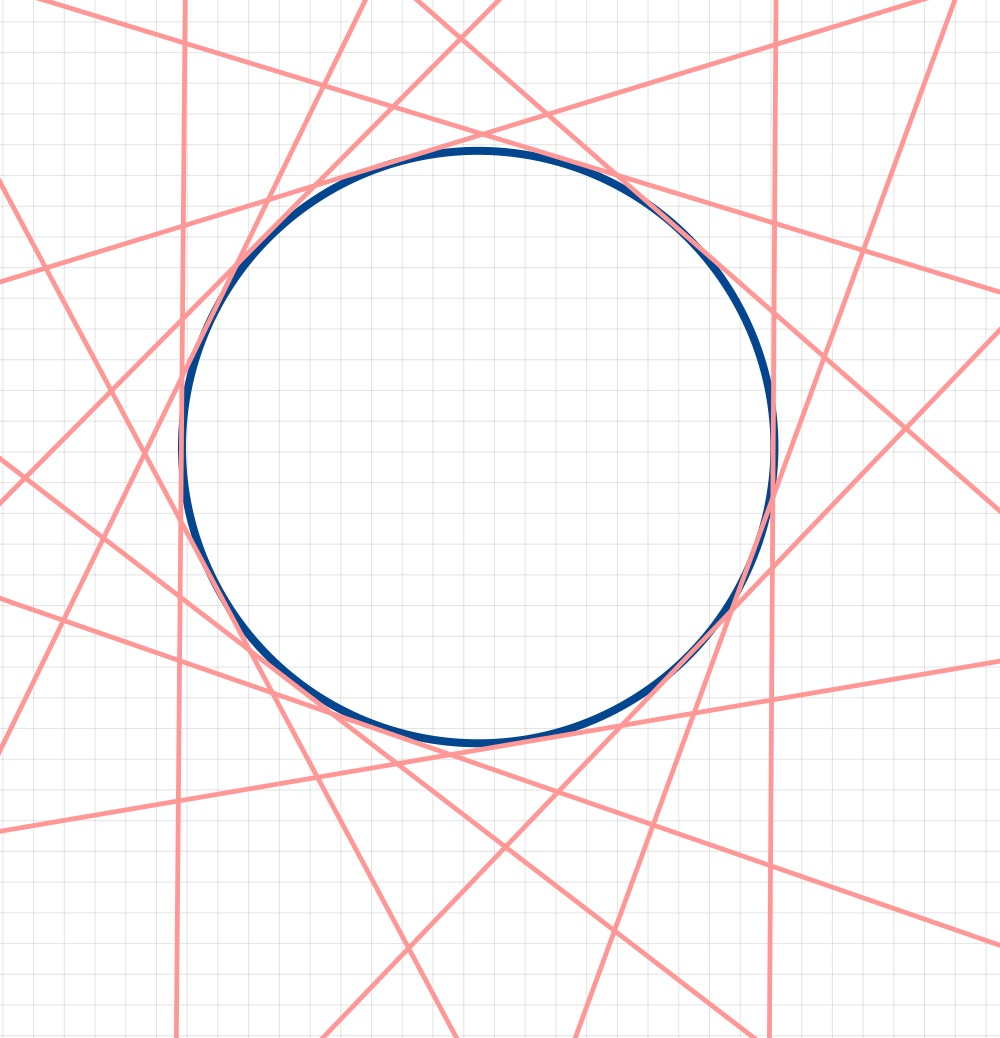
\includegraphics[width=\textwidth]{../\string_build/html/\string_images/bundlea.jpg}
\caption{Visualisierung der Tangentialräume einiger Punkte am Einheitskreises.}\label{\detokenize{manifolds/tangential:fig-bundlea}}\end{figure}

\begin{figure}[htbp]
\centering


\noindent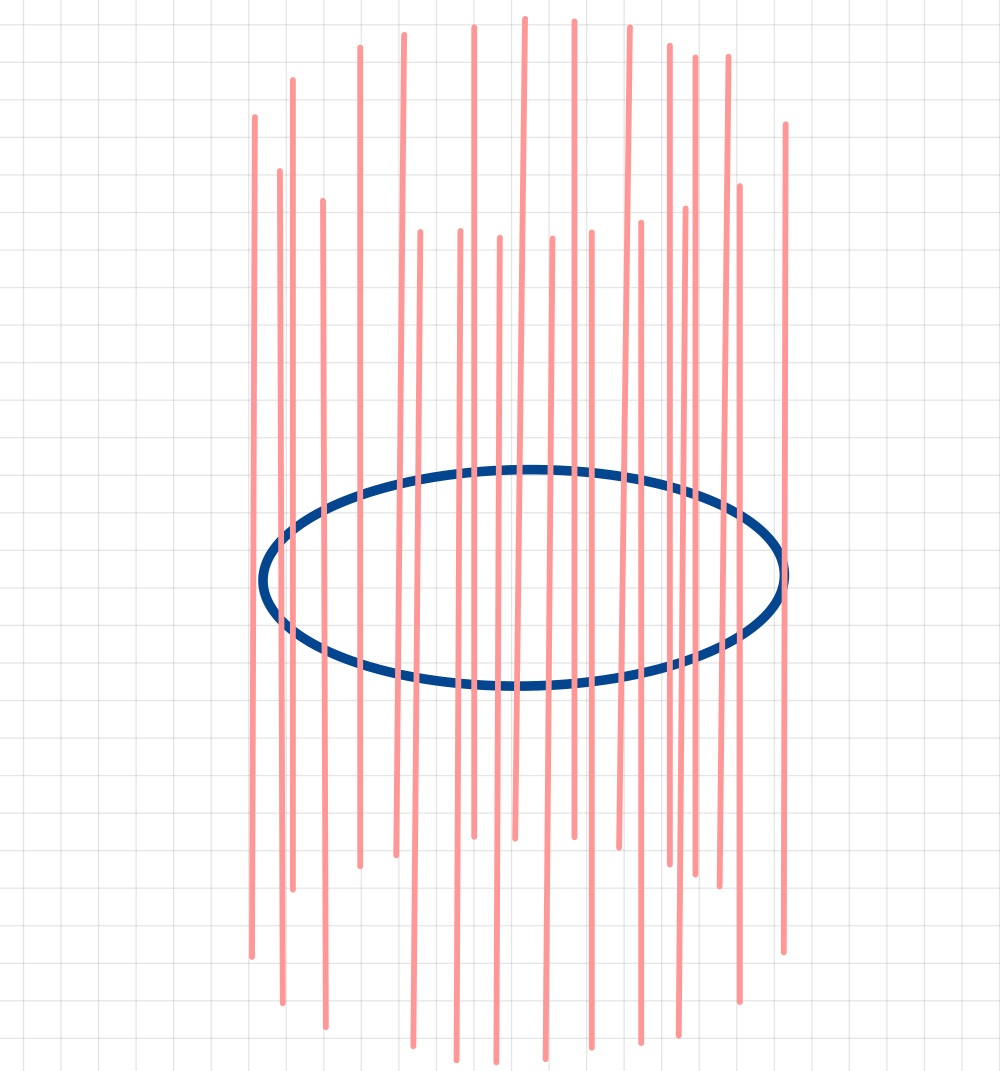
\includegraphics[width=\textwidth]{../\string_build/html/\string_images/bundleb.jpg}
\caption{Visualisierung der disjunkt vereinigten Tangentialräume einiger Punkte am Einheitskreises.}\label{\detokenize{manifolds/tangential:fig-bundleb}}\end{figure}

\par
Wir wollen diese globale Struktur der disjunkten Vereinigung formal definieren.
\begin{definition}{}{manifolds/tangential:definition-20}



\par
Es sei \(\M\) eine glatte Mannigfaltigkeit.
Dann heißt die Menge
\begin{align*}
T\M := \bigsqcup_{p\in\M}  T_p\M = \bigcup_{p\in\M} \{p\} \times T_p\M
\end{align*}
\par
zusammen mit der Projektion
\begin{align*}
\pi:T\M &\to \M\\
\{p\}\times T_p\M &\mapsto p
\end{align*}
\par
das \textbf{Tangentialbündel} von \(\M\).
\end{definition}

\par
Insbesondere erkennen wir, dass wir mit Hilfe der Projektion \(\pi\) jedem Element des Tangentialbündels eindeutig den zu Grunde liegenden Punkt \(p\in\M\) zuordnen können, der den entsprechenden Tangentialraum erzeugt hat.

\par
Im Folgenden wollen wir uns zwei Beispiele für Tangentialbündel an Mannigfaltigkeiten ansehen.
\begin{example}{(Tangentialbündel)}{manifolds/tangential:example-21}





\par
1. Sei \(\M=\R^n\).
Dann ist das Tangentialbündel gerade gegeben durch
\begin{align*}
T\M = \R^n\times\R^n = \R^{2n}.
\end{align*}


\par
2. Wie bereits in \cref{manifolds/tangential:ex:tangentialS1} gesehen erhalten wir für \(\M=\mathbb{S}^1\) als Tangentialbündel den unendlich hohen Zylinder
\begin{align*}
T\M = \mathbb{S}^1\times \R.
\end{align*}\end{example}

\par
In den bisher betrachten Beispielen haben wir als Tangentialbündel jeweils eine Menge der Form \(\M\times \R^n\) erhalten.
Dies ist jedoch nicht immer der Fall wie wir sehen werden.
Tatsächlich bilden Tangentialbündel von dieser Form eine spezielle Unterklasse.
\begin{definition}{}{manifolds/tangential:definition-22}



\par
Sei \(\M\) eine glatte \(n\) dimesnionale Mannigfaltigkeit.
Das Tangentialbündel \(T\M\) heißt \textbf{trivial}, falls gilt
\begin{align*}
T\M\cong \M\times\R^n.
\end{align*}
\par
In diesem Fall nennt man die Mannigfaltigkeit \(\M\) auch \textbf{parallelisierbar}.
\end{definition}
\begin{remark}{}{manifolds/tangential:remark-23}



\par
Es lässt sich zeigen, dass \(\mathbb{S}^1, \mathbb{S}^3,\mathbb{S}^7\) die \emph{einzigen} paralleslisierbaren Sphären sind (siehe \cite{Lee03}).
Die Tatsache, dass \(\mathbb{S}^2\) nicht parallelisierbar ist wird beim Satz vom gekämmten Igel in {prf:ref broken reference}\{TODO\} erneut auftauchen.
\end{remark}

\par
Wir wollen uns nun mit der Frage beschäftigen, wie sich die Tangentialräume für unterschiedliche Punkte \(p,q\in B\) des Basisraums zueinander verhalten, insbesondere wenn \(p\) und \(q\) nahe beieinander liegen.
Hierbei hilft es das abstrakte Konzept eines \textbf{Vektorbündels} zu betrachten.
\begin{definition}{}{manifolds/tangential:definition-24}



\par
Es seien \(\M\) (der sog. Basisraum) und \(E\) (der sog. Totalraum) zwei glatte Mannigfaltigkeiten und \(\pi:E\to \M\) sei glatt und bijektiv. Weiterhin gelte
Außerdem sei \(\pi:E\to \M\) eine glatte und bijektive Abbildung.
Weiterhin gelte
\begin{itemize}
\item {} 
\par
für jeden Punkt \(p\in \M\) sei die sogenannte \textbf{Faser} \(E_p:= \pi^{-1}(p)\) ein \(n\) dimensionaler Vektorraum,

\item {} 
\par
für jeden Punkt \(p\in \M\) existiere eine offene Umgebung \(U\subset \M\) und ein Diffeomorphimus \(\Psi: \pi^{-1}(U)\to U\times\R^n\), so dass für alle \(x\in U\) gilt

\end{itemize}
\begin{align*}
\text{pr}_U(\Psi(x)) &= \pi(x)\quad\forall x\in \pi^{-1}(U)\\
\Psi\rvert_{E_q}&: \pi^{-1}(q) \to \{q\}\times \R^n \text{ ist ein Isomorphismus, für alle }q\in U.
\end{align*}
\par
Dann heißt \((E,\M,\pi)\) \textbf{Vektorbündel} vom Rang \(n\).
Hierbei bezeichnet \(\text{pr}_U(q, z):= q\) die Projektion auf die \(U\) Komponente eines Vektors \((q,z)\in U\times\R^n\).
\end{definition}
\begin{remark}{(Bündel Notation)}{manifolds/tangential:remark-25}



\par
Anstatt das Vektorbündel \((E,\M,\pi)\) als Tripel aufzuschreiben, ist es üblich von einem Bündel \(E\overset{\pi}{\to}\M\) oder sogar \(E\to\M\) zu sprechen.
Die Abbildung \(\pi\) wird im zweiten Fall nur \emph{implizit} vorausgesetzt.
\end{remark}

\par
Die Funktion \(\Psi\) nennt man in diesem Kontext \textbf{lokale Trivialisierung}, denn sie erlaubt es uns den Totalraum \(E\) lokal als Produktraum darzustellen.
Analog zum Tangentialbündel nennen wir ein Vektorbündel \textbf{trivial}, falls eine Trivialsierung \(\Psi:E\to \M\times\R^n\) existiert, so dass gilt
\begin{align*}
E \cong \M\times\R^n.
\end{align*}\begin{example}{}{manifolds/tangential:example-26}



\par
Möbius Band.
\end{example}

\par
Wir wollen nun zeigen, dass das Tangentialbündel ein Vektorbündel ist.
Dazu benötigen wir zunächst die Hilfsaussage des folgenden Lemmas, dass das Tangentialbündel \(T\M\) selbst eine glatte Mannigfaltigkeit ist.
\begin{lemma}{}{manifolds/tangential:lem:tanman}



\par
Es sei \(\M\) eine glatte \(n\) dimensionale Mannigfaltigkeit.
Dann ist das Tangentialbündel \(T\M\) eine glatte \(2n\) dimensionale Mannigfaltigkeit.
Insbesondere ist
\begin{align*}
\pi:T\M &\to \M\\
\{p\}\times T_p\M &\mapsto p
\end{align*}
\par
eine glatte und bijektive Abbildung.
\end{lemma}

\begin{proof}
 Wir werden lediglich die Idee skizzieren, für den vollständingen Beweis siehe Proposition 3.18 in \cite{Lee03}.
Wir benutzen hier die algebraische Definition des Tangentialraums.

\par
Es sei \((U,\varphi)\) eine Karte.
Wir betrachten die Menge \(\pi^{-1}(U)\subset T\M\) und die Abbildung
\begin{align*}
\psi:\pi^{-1}(U) \to \phi(U)\times \R^{n}\subset\R^{2n}\\
(p,v) &\mapsto (\varphi(p), v(\varphi)),
\end{align*}
\par
wobei wir für \(v\in T_p\M\subset (C^\infty(\M))^\ast\) die Notation
\begin{align*}
v(\varphi) := (v(\varphi_1),\ldots, v(\varphi_n))
\end{align*}
\par
benutzt haben.
Es stellt sich dann heraus, dass so definierte Abbildungen \(\psi\) Karten auf \(T\M\) und somit tatsächlich auch eine Mannigfaltigkeit definieren.
Insbsondere ist ein so definiertes \(\psi\) ein Diffeomorphismus.
\end{proof}

\par
Mithilfe der obigen Aussage können wir nun zeigen, dass \(T\M\) ein Vektorbündel ist.
\begin{lemma}{}{manifolds/tangential:lem:tanbundle}



\par
Es sei \(\M\) eine glatte \(n\) dimensionale Mannigfaltigkeit mit dem Tangentialraum
\begin{align*}
T\M:= \bigsqcup_{p\in\M}  T_p\M = \bigcup_{p\in\M} \{p\} \times T_p\M
\end{align*}
\par
und der Abbildung
\begin{align*}
\pi:T\M\to \M\\
\{p\}\times T_p\M\mapsto p.
\end{align*}
\par
Dann ist \((T\M, \M, \pi)\) ein Vektorbündel vom Rang \(n\).
\end{lemma}

\begin{proof}
 Es sei \((U,\varphi)\) eine Karte für \(\M\).
Dann definieren wir die Abbildung
\begin{align*}
\Psi: \pi^{-1}(U) &\to U\times \R^n\\
(p,v) &\mapsto (p, v(\varphi)).
\end{align*}
\par
Wir erkennen sofort, dass \(\Psi\) linear ist und dass \((\text{pr}_U\circ\Psi)(p,v) = p = \pi(p,v)\) gilt.
Da \(\phi\) ein Diffeomorphismus ist, ist
\begin{align*}
\phi\times\text{Id}:U\times \R^n &\to \phi(U)\times\R^n\\
(p,z) &\mapsto (\phi(p), z)
\end{align*}
\par
ebenfalls ein Diffeomorphismus.
Hierbei bemerken wir aber, dass gilt
\begin{align*}
\big((\phi\times\text{Id})\circ \Psi\big)(p,v) = (\phi\times\text{Id})(p, v(\varphi)) = (\phi(p), v(\varphi)).
\end{align*}
\par
Somit entspricht \((\phi\times\text{Id})\circ \Psi\) gerade der Karte aus dem Beweis von \cref{manifolds/tangential:lem:tanman} und ist somit auch ein Diffeomorphismus.
Daraus folgt aber, dass \(\Psi\) schon ein Diffeomorphismus sein muss.
\end{proof}


\subsection{Vektorfelder}
\label{\detokenize{manifolds/tangential:vektorfelder}}
\par
Wir führen zunächst sogenannte Schnitte auf Bündeln ein.
Anschaulich abstrahieren wir hierdurch das Konzept von Funktionsgraphen.
Es sei \(f:\M\to\R^n\) eine vektorwertige Funktion auf einer Mannigfaltigkeit \(\M\).
Dann ist ihr Graph gegeben durch
\begin{align*}
\{(p,f(p)): p\in\M\}\subset \M\times\R^n.
\end{align*}
\par
Hierbei sehen wir, dass \(\M\times\R^n\overset{\pi}{\to}\M\) ein triviales Bündel ist mit
\begin{align*}
\pi(p,(f(p))) = p.
\end{align*}
\par
Verallgemeinert betrachten führt diese Überlegung auf folgende Definition.
\begin{definition}{}{manifolds/tangential:definition-29}



\par
Es sei \(\M\) eine glatte Mannigfaltigkeit und \(E\overset{\pi}{\to}\M\) ein Vektorbündel.
Für eine offene Umgebung \(U\subset\M\) heißt eine glatte Abbildung
\begin{align*}
\sigma: U\to E
\end{align*}
\par
\textbf{lokaler glatter Schnitt}, falls
\begin{align*}
\pi(\sigma(p)) = p\quad\text{ für alle }p\in U.
\end{align*}
\par
Die Menge der glatten Schnitte auf \(U\) wird mit \(\Gamma(E\rvert_U)\) bezeichnet.
Falls die Umgebung \(U\) die ganze Mannigfaltigkeit ist, d.h., es gilt \(U=\M\), dann heißt \(\sigma\) \textbf{glatter Schnitt} und wir definieren \(\Gamma(E):=\Gamma(E\rvert_\M)\).
\end{definition}

\par
Für offenen Mengen im Euklidischen Raum kennen wir bereits den Begriff \textbf{Vektorfeld}.
Hierbei handelt es sich nämlich um eine Funktion
\begin{align*}
F:U\to\R^n,
\end{align*}
\par
wobei \(U\subset\R^n\) eine offene Umgebung ist.
Wir nehmen in diesem Fall also Punkte \(x\in\R^n\) und ordnen ihnen Vektoren \(F(x)\in\R^n\) aus dem gleichen Raum zu.

\par
Betrachten wir statt offener Mengen \(U\subset\R^n\) nun glatte Mannigfaltigkeiten \(\M\), so stellt sich a priori die Frage in welchen Raum Vektorfelder abbilden sollen.
Es stellt sich heraus, dass der Tangentialraum \(T\M\) die richtige Wahl des Zielraums darstellt.
Somit können wir das Konzept von Vektorfeldern verallgemeinern indem wir sie als Schnitte des Tangenialraums auffassen.
\begin{definition}{}{manifolds/tangential:definition-30}



\par
Es sei \(\M\) eine glatte Mannigfaltigkeit.
Wir nennen einen glatten Schnitt
\begin{align*}
X:\M\to T\M
\end{align*}
\par
ein \textbf{glattes Vektorfeld}.
Das Argument von \(X\) wird hierbei meist als Subskript notiert, d.h., \(X_p := X(p)\).
\end{definition}

\par
Für Tangentialbündel haben wir die Abbildung \(\pi:T\M\to\M\) durch
\begin{align*}
\pi(p,v):= p\quad\text{ für } (p,v)\in\{p\}\times T_p\M
\end{align*}
\par
definiert.
Ist \(X\) nun ein glattes Vektorfeld, so gilt
\begin{align*}
\pi(X(p)) = p
\end{align*}
\par
und somit insbesondere \(X_p\in T_p\M\).
Ein Vektorfeld ordnet also jedem Punkt \(p\in\M\) ein Element seines Tangentialraums zu.
Falls \(\M\) eine offene Menge in \(\R^n\) ist, ist dies insbesondere \textbf{konsistent} zur bekannten Definition von Vektorfeldern in Euklidischen Räumen.


\subsubsection{Wirkung von Vektorfeldern}
\label{\detokenize{manifolds/tangential:wirkung-von-vektorfeldern}}
\par
Von der algebraischen Definition des Tangentialraums ist das totale Differential \(df_p\in T^\ast_p\M\) bekannt, welches für \(D\in T^{\text{alg}}_p\M\) und eine Funktion \(f\in C^\infty(M)\) definiert ist durch
\begin{align*}
df_p(D):= D(f).
\end{align*}
\par
Mithilfe dieses mathematischen Werkzeugs können wir nun die Wirkung eines Vektorfelds definieren.
\begin{definition}{}{manifolds/tangential:def:wirkung}



\par
Es sei \(\M\) eine glatte Mannigfaltigkeit und \(X\in\Gamma(T\M)\).
Die \textbf{Wirkung} von \(X\) auf \(C^\infty\) ist definiert durch
\begin{align*}
X(\cdot):C^\infty(M) &\to C^\infty(\M)\\
f &\mapsto [p\mapsto X_p(f) := df_p(X)].
\end{align*}\end{definition}


\subsubsection{Lokale Basis von Vektorfeldern}
\label{\detokenize{manifolds/tangential:lokale-basis-von-vektorfeldern}}
\par
Aus \hyperref[\detokenize{manifolds/tangential:sec-tpbasis}]{Abschnitt \ref{\detokenize{manifolds/tangential:sec-tpbasis}}} wissen wir bereits, dass wir für jeden Punkt \(p\in\M\) die entsprechenden Tangentialvektoren \(v\in T_p\M\) durch die partiellen Derivationen \(\partial_{x^i}^p\) darstellen können.
Im Kontext von Tangentialbündeln stellt sich die natürliche Frage, wie sich diese Vektoren verändern, wenn der Punkt \(p\in\M\) variiert wird.
Hierzu definieren wir zunächst folgende Abbildungen.
\begin{definition}{}{manifolds/tangential:definition-32}



\par
Es sei \(\M\) eine glatte \(n\) dimensionale Mannigfaltigkeit und \((U,\phi)\) eine Karte.
Dann definieren wir die sogenannten \textbf{lokalen Koordinatenfelder} für \(i=1,\ldots,n\) durch
\begin{align*}
\partial_{x^{i}}&:\M\to T\M\\
\partial_{x^{i}}(p)&:= \partial_{x^{i}}\rvert_p.\end{align*}\end{definition}

\par
Mithilfe dieser lokalen Koordinatenfelder können wir nun Vektorfelder lokal darstellen.
\begin{lemma}{}{manifolds/tangential:lem:localsections}



\par
Es sei \(\M\) eine glatte Mannigfaltigkeit und \((U,\phi)\) sei eine Karte von \(\M\).
Dann gilt für \(X\in\Gamma(T\M\rvert_U)\) und die Koeffizientenfunktionen \(X^i:=X(\phi_i)\in C^\infty(U)\), dass gilt
\begin{align*}
X = \sum_{i=1}^n X^i \partial_{x^{i}}.
\end{align*}\end{lemma}

\begin{proof}
 Es sei \(p\in\M\) ein beliebiger Punkt der Mannigfaltigkeit.
Dann haben wir wegen \cref{manifolds/tangential:thm:tanbasis} die Darstellung
\begin{align*}
X_p = \sum_{i=1}^n X_p(\phi_i) \partial_{x^i}^p.
\end{align*}
\par
Mit der \cref{manifolds/tangential:def:wirkung} der Wirkung von Vektorfeldern folgt dann schon
\begin{align*}
X = \sum_{i=1}^n X(\phi_i) \partial_{x^i}.
\end{align*}\end{proof}

\par
Aus der obigen Darstellung folgt auch, dass lokal für eine Karte \((U,\phi)\) die Wirkung auf \(f\in C^\infty(U)\) geschrieben werden kann als
\begin{align*}
X(f) := \sum_{i=1}^n X^i \frac{\partial f}{\partial_{x^i}}.
\end{align*}

\subsection{Das Kotangentialbündel}
\label{\detokenize{manifolds/tangential:das-kotangentialbundel}}\label{\detokenize{manifolds/tangential:s-kotangbundel}}
\par
Analog zum Kotangentialraum, können wir auch das Kotangentialbündel definieren.
\begin{definition}{}{manifolds/tangential:definition-34}



\par
Es sei \(\pi:T\M\to\M\) eine Tangentialbündel, dann ist das \textbf{Kotangentialbündel} \(\pi^\ast: T^\ast\M\to\M\) mit der Menge
\begin{align*}
T^\ast\M := \bigsqcup_{p\in\M} T_p\M
\end{align*}
\par
und der Projektion
\begin{align*}
(\pi^{\ast})^{-1}(p):= \{p\}\times T_p^\ast\M
\end{align*}
\par
definiert.
\end{definition}
\begin{remark}{}{manifolds/tangential:remark-35}



\par
Per Definition ist eine Projektion \(\pi^\ast\) surjektiv und besitzt eine Rechtsinverse \(\pi^\ast\), weshalb obige Definition impliziert, dass für alle \(p\in\M\)
\begin{align*}
\pi({p}\times T_p^\ast\M) = \pi((\pi^{\ast})^{-1}(p)) = p
\end{align*}
\par
gilt. Insbesondere hat aber jedes Element \(x\in T^\ast\M\) eine Darstellung \(x=\{p\}\times T_p^\ast\M\) für ein \(p\in\M\), weshalb man \(\pi\) wie oben angegen tatsächlich über die Inverse definieren kann.
\end{remark}

\par
Auch in diesem Fall erhält man ein Vektorbündel.
\begin{lemma}{}{manifolds/tangential:lemma-36}



\par
Es sei \(\pi:T\M\to\M\) eine Tangentialbündel, dann ist das Kotangentialbündel \(\pi^\ast:T^\ast\M\to\M\) ein Vektorbündel.
\end{lemma}

\begin{proof}
 Der Beweis funktioniert analog zum Beweis von \cref{manifolds/tangential:lem:tanbundle}  Für die Details zur Argumentation weshalb auch \(T^\ast\M\) eine Mannigfaltigkeit ist, verweisen wir auf \cite{Lee03} Prop. 11.9.
\end{proof}

\par
Wir interessieren uns auch hier für glatte Schnitte, welche in diesem Kontext als 1 Differentialformen bezeichnet werden.
\begin{definition}{}{manifolds/tangential:definition-37}



\par
Ein glatter Schnitt \(\omega\in\Gamma(T^\ast\M)\) wir als 1 Differentialform bezeichnet, zusätzlich benutzen wir die Notation
\begin{align*}
\Omega^1(\M) := \Gamma(T^\ast\M)
\end{align*}\end{definition}

\par
Man kann hier analog lokale Koordinaten Kovektorfelder definierne indem man lokale Koordinaten betrachtet und die duale Basisdarstellung des Kotangentialraums benutzt.
\begin{definition}{}{manifolds/tangential:definition-38}



\par
Es sei \(\M\) eine glatte \(n\) dimensionale Mannigfaltigkeit und \((U,\phi)\) eine Karte.
Dann definieren wir die sogenannten \textbf{lokalen Koordinaten Kovektorfelder} für \(i=1,\ldots,n\) durch
\begin{align*}
dx^{i}:\M&\to T\M\\
p&\mapsto dx^{i}_p.\end{align*}\end{definition}

\par
Die definierten 1 Formen sind die einfachsten Beispiele der allgmeinen Diffenerentialformen, welche wir in \hyperref[\detokenize{manifolds/diffformen:s-difformen}]{Abschnitt \ref{\detokenize{manifolds/diffformen:s-difformen}}} untersuchen werden. Das Konzept des Kotangentialbündels und der Differentialform ist nun noch etwas abstrakt, allerdings erhalten wir mithilfe des totalen Differentials \cref{manifolds/tangential:def:totdiff} erneut eine einfache Veranschalichung.
\begin{example}{}{manifolds/tangential:ex:totdiff}



\par
Es sei \(\M\) eine glatte Mannigfaltigkeit und \(f\in C^\infty(\M)\), dann ist die Abbildung
\begin{align*}
df:\M\to T^\ast\M\\
p\mapsto (p, df_p)
\end{align*}
\par
eine Differentialform, wobei \(df_p\in T_p^\ast\M\) für eine Derivation \(D\in T_p\M\) definiert ist durch
\begin{align*}
df_p(D) := D(f),
\end{align*}
\par
weil \(D\) als Derivation gerade eine lineare Abbildung \(D:C^\infty\to\R\) ist.

\par
Für die Glattheitseigenschaft verweisen wir auf \cite{Lee03} Prop. 10.22., was zeigt, dass \(df\) eine glatte Abbildung ist. Desweiteren sehen wir, dass
\begin{align*}
\pi^\ast(df(p)) = \pi^\ast((p,df_p)) = p\end{align*}
\par
und somit gilt per Definition diese Eigenschaft eines Schnittes. Sei nun \((U,\varphi)\) eine Karte mit lokalen Koordinaten \(\varphi = (x^1,\ldots, x^n)\). Für \(p\in\M\) und \(D\in T_p\M\) Derivation gilt nach ??, dass
\begin{align*}
D = \sum_{i=1}^n D(x^i)\, \partial_{x^i}^p = \sum_{i=1}^n dx^{i}(D)\, \partial_{x^i}^p,
\end{align*}
\par
wobei hierbei \(dx^{i}:T_p\M\to\R\) eine Element der dualen Basis ist. Daraus folgt für das totale Differential an \(p\), \(df_p:T_p\M\to\R\), per Defintion dass
\begin{align*}
df_p(D) = \sum_{i=1}^n dx_p^{i}(D)\, df_p(\partial_{x^i}^p) = 
\sum_{i=1}^n dx_p^{i}(D)\, \partial_{x^i}^p(f)
\end{align*}
\par
gilt. Somit gilt also lokal in \(U\)
\begin{align*}
df = \sum_{i=1}^n dx^{i}\, \partial_{x^i}(f).
\end{align*}\end{example}

\par
Für den Fall, dass die Mannigfaltigkeit \(\M\) eine offene Teilmene des \(\R^n\) ist erhalten wir einen einfachen Zusammenhang zur klassischen Richtungsableitung.
\begin{example}{}{manifolds/tangential:example-40}



\par
Es sei \(\M=U\subset\R^n\) eine offene Teilmenge, für jedes \(p\in\M\) können wir den Tangentialraum dann mit dem \(\R^n\) identifizieren und erhalten, dass das totale Differential an \(p\) gegeben ist durch
\begin{align*}
df_p:\R^n&\to\R\\
v&\mapsto \langle \nabla f(p), v \rangle = \sum_{i=1}^n \partial_i f(p)\, v^i.
\end{align*}
\par
Insbsondere ist \(dx^{i}\) in diesem Fall die Funktion welche einen Vektor auf seine Komponenten abbildet, somit gilt
\begin{align*}
dx^{i}(v) = v^i
\end{align*}
\par
und daher insgesamt wiederum
\begin{align*}
df = \sum_{i=1}^n \partial_i f, dx^{i}.
\end{align*}\end{example}

\par
Zusätzlich haben wir hier auch eine lokale Basisdarstellung als analoges Resultat zu \cref{manifolds/tangential:lem:localsections} hier nun aber mit den Basiselementen des Kotangentialraums, bzw. den lokalen Koordinaten Kovektorfeldern.
\begin{lemma}{}{manifolds/tangential:lem:coordcovec}



\par
Es sei \(\M\) eine glatte \(n\) dimensionale Mannigfaltigkeit und \((U,\phi)\) eine Karte mit lokalen Koordinaten \(\varphi=(x^1,\ldots, x^n)\),  dann gilt für jede Differentialform \(\omega\in\Omega^1(U)\), dass
\begin{align*}
\omega = \sum_{i=1}^n f_i dx^i
\end{align*}
\par
wobei \(f_i\in C^\infty(\M)\) gegeben ist durch \(\omega(\partial_{x^i})\).
\end{lemma}

\begin{proof}
 Siehe z.B. \cite{Lee03} Seite 282.
\end{proof}


\subsection{Tensorfelder}
\label{\detokenize{manifolds/tangential:tensorfelder}}
\par
Als natürliche Verallgemeinerung wollen wir nun das Konzept der Felder auf Mannigfaltigkeiten von Vektoren auf Tensoren übertragen. Um ein Tensorfeld definieren zu können müssen wir zunächst klären, wie das Tensorprodukt von Tangentialbündeln aussehen soll. Für zwei Vektorbündel \(E\overset{\pi_E}{\to}{\M}, F\overset{\pi_F}{\to}{\M}\) wissen wir, dass für jedes \(p\in\M\) die Fasern \(E_p, F_p\) endlichdimensionale Vektorräume sind. Insbeonsdere können wir also das Tensorprodukt
\begin{align*}
E_p\otimes F_p
\end{align*}
\par
betrachten und damit ein Bündel auf dem Totalraum
\begin{align*}
E\otimes F:= \bigsqcup_{p\in\M} E_p\otimes F_p
\end{align*}
\par
betrachten. Die entsprechende Projektion \(\pi_{E\otimes F}:E\otimes F\to\M\) ist gegeben durch
\begin{align*}
\pi_{E\otimes F}^{-1}(p):= E_p\otimes F_p := (E\otimes F)_p.
\end{align*}\begin{lemma}{}{manifolds/tangential:lem:tensorbundle}



\par
Es sei \(E\overset{\pi_E}{\to}{\M}\) ein Vektorbündel vom Rang \(k\) und \(F\overset{\pi_F}{\to}{\M}\) ein Vektorbündel vom Rang \(l\), dann ist
\begin{align*}
\pi_{E\otimes F}:(E\otimes F)\to \M
\end{align*}
\par
ein Vektorbündel vom Rang \(kl\).
\end{lemma}

\begin{proof}
 Siehe Übung.
\end{proof}

\par
Die Definition des Tensorbündels lässt sich direkt auf mehrfache Tensorprodukte übertragen und führt uns direkt auf gemischte Tensorbündel.
\begin{definition}{}{manifolds/tangential:definition-43}



\par
Es sei \(\M\) eine glatte Mannigfaltigkeit, und \(r,s\in\N_0\), s.d. \(r+s>0\), dann heißt
\begin{align*}
T^r_s\M := \bigsqcup_{p\in\M} T^r_s(T_p\M) \to \M
\end{align*}
\par
Tensorbündel der Stufe \((r,s)\).
\end{definition}

\par
Mit den vorherigen Überlegungen können wir direkt schlussfolgern, dass wir hier erneut ein Vektorbündel definiert haben. Insbesondere, da nach \cref{vektoranalysis/tensor:cor:tensorMultilinearform} \begin{align*}
T^r_s(T_p\M) \cong \underbrace{T_p\M\otimes\ldots T_p\M}_{r\text{ mal}}\otimes\underbrace{T_p^ast\M\otimes\ldots T_p\ast\M}_{s\text{ mal}}
\end{align*}
\par
gilt erhalten wir die Bündelstruktur über Anwendung von \cref{manifolds/tangential:lem:tensorbundle} 
\label{manifolds/tangential:corollary-44}
\begin{emphBox}{}{}{Corollary 4.1}



\par
Es sei \(\M\) eine glatte Mannigfaltigkeit, und \(r,s\in\N_0\), s.d. \(r+s>0\), dann ist \(\pi:T^r_s\M\to\M\) mit der kanonisch nach \cref{manifolds/tangential:lem:tensorbundle} definierten Abbildung \(\pi\) ein Vektorbündel.
\end{emphBox}

\begin{proof}
 Folgt direkt aus \cref{manifolds/tangential:lem:tensorbundle} 
\end{proof}

\par
Da wir die Struktur eines Vektorbündels definiert haben können wir nun auf natürliche Weise auch \textbf{Tensorfelder} als glatte Schnitte definieren.
\begin{definition}{}{manifolds/tangential:definition-45}



\par
Es sei \(\M\) eine glatte Mannigfaltigkeit, und \(r,s\in\N_0\), s.d. \(r+s>0\), ein \textbf{Tensorfeld} ist ein glatter Schnitt \(A\in \Gamma(T^r_s\M)\).
\end{definition}

\par
Dank der lokalen Darstellung von Vektorbündeln in \cref{manifolds/tangential:lem:localsections} können wir die recht abstrakten Tensorfelder lokal sehr konkret Darstellen.
\label{manifolds/tangential:cor:tensorfieldchart}
\begin{emphBox}{}{}{Corollary 4.2}



\par
Es sei \(\M\) eine glatte \(n\) dimensionale Mannigfaltigkeit, \((U,\varphi)\) eine Karte mit lokalen Koordinaten \(\varphi=(x^1,\ldots,x^n)\). Für \(r,s\in\N_0\), s.d. \(r+s>0\) und \(A\in \Gamma(T^r_s\M)\) ein Tensorfeld existieren glatte Koeffizientenfunktionen \(A^{i_1,\ldots, i_s}_{j_1,\ldots,j_r}\in C^\infty(\M)\) für \(i_1,\ldots, i_s, j_1,\ldots, j_r\in \{1,\ldots,n\}\), s.d.,
\begin{align*}
A = A^{i_1,\ldots,i_s}_{j_1,\ldots,j_r} \partial_{x_{i_1}}\otimes\ldots\otimes \partial_{x_{i_r}}\otimes dx^{j_1}\otimes\ldots\otimes dx^{j_s}.
\end{align*}\end{emphBox}

\begin{proof}
 Folgt aus \cref{manifolds/tangential:lem:localsections} und \cref{manifolds/tangential:lem:coordcovec}   für Details siehe \cite{Lee03} Prop. 12.19.
\end{proof}

\par
Ähnlich zu den Überlegungen in \hyperref[\detokenize{vektoranalysis/tensor:s-symtensoren}]{Abschnitt \ref{\detokenize{vektoranalysis/tensor:s-symtensoren}}} können wir auch hier das Tensorprodukt von Tensorfeldern betrachten.
\begin{lemma}{}{manifolds/tangential:lemma-47}



\par
Es sei \(\M\) eine glatte Mannigfaltigkeit, für \(r,l\in \N\) seien \(A\in \Gamma(T^r_0\M), B\in \Gamma(T^l_0\M)\) zwei Tensorfelder und \(f\in C^\infty(\M)\), dann sind \(fA\) und \(A\otimes B\) Tensorfelder mit lokalen Koeffezienten
\begin{align*}
(fA)_{i_1,\ldots i_{k}} = f A_{i_1,\ldots, i_k}\\
(A\otimes B)_{i_1,\ldots,i_{l+r}} = A_{i_1,\ldots, i_l} B_{i_{l+1},\ldots, i_{l+k}}.
\end{align*}\end{lemma}

\begin{proof}
 Siehe \cite{Lee03} Prop. 12.22.
\end{proof}


\section{Differentialformen auf Mannigfaltigkeiten}
\label{\detokenize{manifolds/diffformen:differentialformen-auf-mannigfaltigkeiten}}\label{\detokenize{manifolds/diffformen::doc}}
\par
Die vorhergehenden Abschnitte liefern nun die nötigen Grundlagen um \textbf{Differentialformen} zu betrachten. Insbesondere werden wir diese über eine Unterstruktur der bekannten Tensorfelder erhalten. Dieser Schritt isr konzeptionell sehr ähnlich zum Schritt von allgemeinen Tensoren zu den Antisymmetrischen, bzw. alternierenden Tensoren. Dieser Zusammenhang erklärt auch die Begrifflichkeit alternierende Differentialform welche in de Literatur häufig vorkommt.

\par
Differentialformen sind ein wichtiges Konzept in verschieden Bereichen der Mathematik und Physik. Auch wenn wir diese Thematik hier nicht betrachten, sei erwähnt, dass Differentialformen die Integration auf speziellen glatten Mannigfaltigkeiten erlauben.


\subsection{Differentialformen}
\label{\detokenize{manifolds/diffformen:differentialformen}}\label{\detokenize{manifolds/diffformen:s-difformen}}
\par
In Kapitel ?? haben wir symmetrische und antisymmetrische Tensoren kennengelernt. Dieses Konzept werden wir nun auf Tensorfelder übetragen um somit Differntialformen zu erhalten. Hierfür betrachten wir für eine glatte Mannigfaltigkeit die Menge
\begin{align*}
\Lambda^k T^\ast\M := \bigsqcup_{p\in\M} \Lambda^k (T^\ast_p\M)
\end{align*}
\par
der alternierenden Tensorfelder. Antisymmetrische Tensoren bilden direkt eine Teilmenge aller Tensoren und es bleibt lediglich zu zeigen, dass die Vektorraumstruktur erhalten bleibt. Die Situation hier ist nun anders, man benötigt den abstrakten Begriff des \textbf{Untervektorbündels}.
\begin{definition}{}{manifolds/diffformen:definition-0}



\par
Es seien \(\pi_E:E\to B\) und \(\pi_D:D\to B\) zwei Vektorbündel, wobei für jedes \(p\in\M\) die Untervektorraumrelation
\begin{align*}
\pi_D^{-1}(p) = D_p\subset E_p = \pi_E^{-1}(p)
\end{align*}
\par
gelte, dann heißt \(D\) Untervektorbündel von \(E\).
\end{definition}

\begin{figure}[htbp]
\centering


\noindent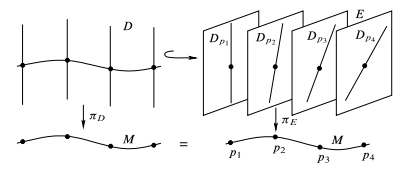
\includegraphics[width=\textwidth]{../\string_build/html/\string_images/subbundle.png}
\caption{Visualisierung eines Untervektorbündels, siehe Kapitel 10 in \cite{Lee03}.}\label{\detokenize{manifolds/diffformen:fig-subbundle}}\end{figure}

\par
In diesem Fall erhält man also ein Untervektorbündel.
\begin{lemma}{}{manifolds/diffformen:lemma-1}



\par
Sei \(\M\) eine glatte \(n\) dimensionale Mannigfaltigkeit, dann ist \(\Lambda^k T^\ast\M\) ein glattes Untervektorbündel vom Rang \(\begin{pmatrix} n k \end{pmatrix}\).
\end{lemma}

\begin{proof}
 ToDo.
\end{proof}

\par
Dank der Bündelstruktur können wir erneut glatte Schnitte betrachten, welche nun auf das Konzept der Differentialform führen.
\begin{definition}{}{manifolds/diffformen:definition-2}



\par
Es sei \(\M\) eine glatte Mannigfaltigkeit, dann nennt man einen glatten Schnitt
\begin{align*}
\omega\in \Gamma(\Lambda^k T^\ast\M)
\end{align*}
\par
eine \(k\) Differentialform oder auch \(k\) Form. Den Vektorraum der Differentialformen notieren wir durch
\begin{align*}
\Omega^k(\M) := \Gamma(\Lambda^k T^\ast\M).
\end{align*}\end{definition}


\subsection{Das äußere Produkt}
\label{\detokenize{manifolds/diffformen:das-auszere-produkt}}
\par
In \hyperref[\detokenize{vektoranalysis/tensor:s-symtensoren}]{Abschnitt \ref{\detokenize{vektoranalysis/tensor:s-symtensoren}}} haben wir das äußere Produkt \(\wedge\) kennengelernt, welches wir nun auf Differentialformen übertragen. Dazu seien \(\omega\in \Omega^k(\M), \eta\in \Omega^l(\M)\) zwei Differentialformen für \(k,l\in\N\), dann setzten wir
\begin{align*}
\omega \wedge \eta:\M &\to \Lambda^{k+l}T^\ast\M\\
p&\mapsto \omega_p \wedge \eta_p
\end{align*}
\par
was in der Tat eine Differentialform definiert, also \(\omega\wedge\eta \in \Omega^{k+l}(\M)\). Zusätzlich überträgt sich auch die Darstellung in einer lokalen Karte von \cref{manifolds/tangential:cor:tensorfieldchart} auf diese Situation, wobei das Tensorprodukt, durch das äußere Produkt ersetzt werden kann.
\begin{lemma}{}{manifolds/diffformen:lemma-3}



\par
Es sei \(\M\) eine glatte Mannigfaltigkeit, \((\varphi,U)\) eine Karte und \(\omega\in\Omega^l(\M)\) eine Differentialform, dann gilt lokal in \(U\)
\begin{align*}
\omega = \sum_{1\leq i_1,\ldots,i_k \leq n}\omega_{i_1\ldots i_k}
dx_{i_1}\wedge\ldots\wedge dx_{i_k},
\end{align*}
\par
wobei \(\omega_{i_1\ldots i_k}\in C^\infty(\M)\) für alle \(i_1,\ldots,i_k\in\{1,\ldots,n\}\) gilts
\end{lemma}

\begin{proof}
 Siehe z.B. \cite{Lee03} Kapitel 14.
\end{proof}
\begin{example}{}{manifolds/diffformen:example-4}



\par
1. Für \(k=0\) und \(\M\) eine glatte Mannigfaltigkeit erhalten wir
\begin{align*}
\Omega^0(\M) = C^\infty(\M).
\end{align*}


\par
2. Für \(k=1\) und \(\M\) eine glatte Mannigfaltigkeit erhalten wir
\begin{align*}
\Omega^1(\M)
\end{align*}
\par
gerade die Kovektorfelder aus \hyperref[\detokenize{manifolds/tangential:s-kotangbundel}]{Abschnitt \ref{\detokenize{manifolds/tangential:s-kotangbundel}}}.



\par
3. Für \(k=3\) und \(\M=\R^3\) ist z.B.,
\begin{align*}
\omega(xy) := \sin(xy) dx\wedge dy
\end{align*}
\par
eine Differentialform.
\end{example}


\subsection{Die äußere Ableitung}
\label{\detokenize{manifolds/diffformen:die-auszere-ableitung}}
\par
Wir wenden uns nun einer wichtigen Operation auf Differentialformen zu, der äußeren Ableitung. Aus \cref{manifolds/tangential:ex:totdiff} kennen wir schon das totale Differential \(df\in \Omega^1(\M)\), für eine glatte Funktion \(f\in C^\infty(\M)\). Hierbei haben wir für ein glattes Vektorfeld \(X\in \Gamma(T\M)\) die Abbildung
\begin{align*}
df(X) := X(f)
\end{align*}
\par
definiert, wobei die rechte Seite über die Wirkung des Vektorfelds definiert ist. Wir können dieses Konzept verallgemeinern, indem wir die äußere Ableitung definieren.
\begin{definition}{}{manifolds/diffformen:definition-5}



\par
Es sei \(\M\) eine glatte Mannigfaltigkeit und \(f\in C^\infty(\M)\), dann definieren wir die lineare Abbildung
\begin{align*}
d:\Omega^k(\M)\to \Omega^{k+1}(\M)\\
d(f\, dx^{i_1}\wedge\ldots\wedge dx^{i_k}):= df \wedge dx^{i_1}\wedge\ldots\wedge dx^{i_k}.
\end{align*}\end{definition}
\begin{remark}{}{manifolds/diffformen:remark-6}



\par
Beachte, dass die obige Abbildung nur jeweils für lokale Koordinaten definiert ist. Wegen der Kartenunabängigkeit führt dies aber auf eine eindeutig definierte Funktion, siehe z.B. \cite{Lee03} Kapitel 14. Da wir \(d\) auf den Elementen \(dx^{i_1}\wedge\ldots\wedge dx^{i_k}\) definiert haben erhalten wir jeweils lokal eine eindeutige lineare Fortsetzung, da jedes \(\omega\in \Omega^k(\M)\) lokal die Darstellung
\begin{align*}
\omega = \sum_{1\leq i_1,\ldots,i_k \leq n}\omega_{i_1\ldots i_k}
dx_{i_1}\wedge\ldots\wedge dx_{i_k}
\end{align*}
\par
hat und somit
\begin{align*}
d\omega &= \sum_{1\leq i_1,\ldots,i_k \leq n} d(\omega_{i_1\ldots i_k}
dx_{i_1}\wedge\ldots\wedge dx_{i_k})\\ 
&= \sum_{1\leq i_1,\ldots,i_k \leq n} d(\omega_{i_1\ldots i_k})\wedge
dx_{i_1}\wedge\ldots\wedge dx_{i_k}
\end{align*}\end{remark}
\begin{example}{}{manifolds/diffformen:ex:10.14}



\par
1. Für \(\omega\in\Omega^0(\R^3)\) ist \(d\omega = \frac{\partial\omega}{\partial x_1}dx_1+
\frac{\partial\omega}{\partial x_2}dx_2+\frac{\partial\omega}{\partial x_3}dx_3\).



\par
2. Für \(\omega = \omega_1dx_1+\omega_2dx_2+\omega_3dx_3\in\Omega^1(\R^3)\) ist
\begin{align*}
d\omega &=& (d\omega_1)\wedge dx_1+(d\omega_2)\wedge dx_2+(d\omega_3)\wedge
dx_3\\
&=& \left(\frac{\partial\omega_2}{\partial x_1}-\frac{\partial\omega_1}{\partial x_2}\right)
dx_1\wedge dx_2+ \left(\frac{\partial\omega_3}{\partial x_2}-\frac{\partial\omega_2}{\partial x_3}\right)
dx_2\wedge dx_3\\
&& + \left(\frac{\partial\omega_1}{\partial x_3}-\frac{\partial\omega_3}{\partial x_1}\right)
dx_3\wedge dx_1.
\end{align*}


\par
3. Für \(\omega = \omega_{12}dx_1\wedge dx_2+\omega_{23}dx_2\wedge dx_3
+\omega_{31}dx_3\wedge dx_1 \in\Omega^2(\R^3)\) ist
\begin{align*}
d\omega = \left(\frac{\partial\omega_{12}}{\partial x_3} + \frac{\partial\omega_{23}}{\partial x_1}
+ \frac{\partial\omega_{31}}{\partial x_2}\right)dx_1\wedge dx_2\wedge dx_3.
\end{align*}


\par
4. Für \(\omega\in\Omega^3(\R^3)\) ist \(d\omega=0\).
\end{example}

\par
Für die äußere Ableitung können wir zusätzlich folgende Eigenschaften zeigen.
\begin{lemma}{}{manifolds/diffformen:lem:outeprop}



\par
Es sei \(\M\) eine glatte Mannigfaltigkeit, dann haben wir folgende Eigenschaften.



\par
1. Für \(f,g\in C^\infty(\M)\) gilt
\begin{align*}
d(fg) = d(f)\,g + f\, d(g).
\end{align*}


\par
2. Für \(\omega\in\Omega^k(\M),\eta\in\Omega^l(\M)\) gilt
\begin{align*}
d(\omega\wedge\eta) = (d\omega)\wedge \eta + (-1)^k \omega\wedge (d\eta).
\end{align*}


\par
3. Es gilt \(d\circ d = 0\).
\end{lemma}
\begin{remark}{}{manifolds/diffformen:remark-9}



\par
Da \(d\) Eigenschaft 2 erfüllt, nennt man \(d\) auch Antiderivation.
\end{remark}

\par
Eine interessante Anwendung finden Differntialformen im sog. Poincaré Lemma. Hierfür benötigen wir folgenden Begriffe
\begin{definition}{}{manifolds/diffformen:def:geschlossenexakt}



\par
Es sei \(\M\) eine glatte Mannigfaltigkeit, eine Differentialform \(v\in\Omega^k(\M)\) heißt
\begin{itemize}
\item {} 
\par
\textbf{geschlossen}, wenn \(dv=0\),

\item {} 
\par
\textbf{exakt}, wenn \(v=d\eta\) für ein \(\eta\in\Omega^{k-1}(\M)\) gilt.

\end{itemize}
\end{definition}

\par
Nach Satz {lem:outer:prop broken reference} sind exakte Differentialformen geschlossen, da für \(v=d\eta\) gilt,
\begin{align*}
dv = d(d\eta) = (d\circ d)\eta = 0.
\end{align*}
\par
Das Poincaré Lemma besagt nun, dass auf sternförmigen offenen Mengen \(U\subseteq \R^n\) auch die Umkehrung gilt.
\begin{lemma}{}{manifolds/diffformen:lemma-11}



\par
Es sei \(U\subset\R^n\) eine offene sternförmige Menge, dann gilt für \(\omega\in \Omega^k(\M)\),
\begin{align*}
\omega\text{ ist geschlossen}\Leftrightarrow \omega\text{ ist exakt.}
\end{align*}\end{lemma}

\begin{proof}
 Siehe z.B. \cite{Lee03} Theorem 11.49.
\end{proof}


\subsection{Der Pullback}
\label{\detokenize{manifolds/diffformen:der-pullback}}
\par
Die letzte Operation die wir in diesem Kapitel betrachten ist der sogenannte \textbf{Pullback}. Hierbei betrachten wir zwei glatte Mannigfaltigkeiten \(\M,\mathcal{N}\) und eine glatte Funktion \(F:M\to\mathcal{N}\). Das Ziel ist es nun eine Differentialform auf \(N\), \(\omega\in\Omega^k(\mathcal{N})\) mithilfe von \(F\) auf eine Differentialform auf \(\M\) zurückzuziehen. Ausgewertet an \(p\in\M\) ergibt eine Differentialform \(\eta\in\Omega^k(\M)\) ein Element aus \(L^k(T_p^\ast\M)\),
\begin{align*}
\eta_p\in \Omega^k(T_p\M) \subset L^k(T_p^\ast\M)
\end{align*}
\par
also eine Linearform, welche auf \(k\) Elemente \(v_1,\ldots,v_k\in T_p^\ast\M\) des Kotangentialraums in \(p\) an \(\M\) wirkt. Haben wir nun a priori \(\omega\in\Omega^k(\mathcal{N})\) gegeben brauchen wir deshalb zunächst eine Methode mit der wir Tangentialvektoren über \(F\) von \(\M\) nach \(\N\) vorschieben können, der sogennante \textbf{Pushforward}.
\begin{definition}{}{manifolds/diffformen:definition-12}



\par
Es seien \(\M,\mathcal{N}\) zwei glatte Mannigfaltigkeiten und \(F\in C^\infty(\M,\mathcal{N})\), dann definieren wir für \(p\in\M\)
\begin{align*}
F_\ast:T_p\M\to T_{F(p)}\mathcal{N}\\
D\mapsto \big[f\mapsto D(f\circ F)]
\end{align*}
\par
den sogenannten \textbf{Pushforward}.
\end{definition}

\par
Da wir nun Tangentialvektoren von \(T_p\M\) auf \(T_{F(p)}\mathcal{N}\) schieben können, sind wir in der Lage damit den Pullback von Kotangentialvektoren zu definieren.
\begin{definition}{}{manifolds/diffformen:definition-13}



\par
Es seien \(\M,\mathcal{N}\) zwei glatte Mannigfaltigkeiten und \(F\in C^\infty(\M,\mathcal{N})\), dann definieren wir für \(p\in\M\)
\begin{align*}
F^\ast: T_{F(p)}^\ast\mathcal{N}\to \big[T^p_\M\mapsto\R\big]\\
v \mapsto \big[D\mapsto v(F_\ast(D)) \big]
\end{align*}
\par
den \textbf{Pullback}
\end{definition}
\begin{remark}{}{manifolds/diffformen:remark-14}



\par
Es gilt insbesondere, dass \(F^\ast v \in T_p^\ast\M\) für jedes \(v\in T_{F(p)}^\ast\mathcal{N}\).
\end{remark}

\par
Dieses Konzept können wir nun auf Formen übertragen in dem wir eine neue Differentialform punktweise an \(p\) definieren am Punkt \(F(p)\). Konkret seien \(v_1,\ldots, v_k\in T_p\M\), dann definiere
\begin{align*}
(F^\ast\omega)_p (v_1,\ldots,v_k) := \omega_F(p)\big(F_\ast(v_1),\ldots,F_\ast(v_k)\big).
\end{align*}
\par
Die so definierte Abbildung bildet tatsächlich zwischen den passenden Räumen ab
\begin{align*}
F^\ast:\Omega^k(\mathcal{N})\to\Omega^k(\mathcal{M})\\
\omega\mapsto \big[ p\mapsto (F^\ast\omega)_p \big].
\end{align*}
\par
Zusätzlich erhält man folgende Eigenschaften.
\begin{lemma}{}{manifolds/diffformen:lem:pullbackprop}



\par
Es seien \(\M,\mathcal{N}\) glatte Mannigfaltigkeiten und \(F\in C^\infty(\M,\mathcal{N})\), dann gilt,
\begin{enumerate}

\item {} 
\par
\(F^\ast\) ist linear,

\item {} 
\par
\(F^\ast(\omega\wedge\eta) = F^\ast(\omega) \wedge F^\ast(\eta)\) für \(\omega,\eta\in\Omega^k(\mathcal{N})\).

\item {} 
\par
Für lokale Koordinaten Kovektorfelder \(dy^1,\ldots,dy^m\) und \(f\in C^\infty(\mathcal{N})\) gilt

\end{enumerate}
\begin{align*}
F^\ast(f dy^{i_1}\wedge\ldots\wedge dy^{i_k}) = (f \circ F) d(y^{i_1}\circ F)\wedge\ldots\wedge d(y^{i_k}\circ F).
\end{align*}\end{lemma}

\begin{proof}
 Für 1. und 2. siehe Hausaufgaben, Für 3. siehe \cite{Lee03} Lemma 14.16.
\end{proof}

\par
Im Falle, dass die Mannigfaltigkeiten gleich dem \(\R^n\) bzw. \(\R^m\) sind, also \(\M=\R^n, \mathcal{N}=\R^m\) können wir den Pullback leicht explizit berechnen. Dazu sei \(F:\R^n\to\R^m\) eine glatte Abbildung, \(x_1,\ldots,x_n\) seien Koordinaten für \(\R^n\) und \(y_1,\ldots,y_m\) seien Koordinaten für \(\R^m\).

\par
Zunächst erkennen wir für den Pushforward, \(F_\ast:T_p\M\to T_{F(p)}\mathcal{N}\) dass für \(p\in\M\) gilt,
\begin{align*}
F_\ast(\partial_{x_i^p}) = \sum_{j=1}^m \partial_i F_j\, \partial_{y_j^{F(p)}}
\end{align*}
\par
wobei \(\partial_i F_j\) die \(i\) te partielle Ableitung (im klassichen Sinne) der \(j\) ten Komponente von \(F\) ist.

\par
Betrachten wir also den Pullback eines Kovektorfeldes \(dy^k\) ausgewertet an einem Tangentialvektor \(D\in T_p\M\)
\begin{align*}
D = \sum_{i=^1}^n dx_i^p(D)\, \partial_{x_i^p}
\end{align*}
\par
erhalten wir unter Ausnutzung der Linearität
\begin{align*}
F^\ast(dy^k)_{p}(D) &= dy^k(F_\ast(D)) = 
dy^k\big(\sum_{i=^1}^n dx_i^p(D)\, F^\ast(\partial_{x_i^p})\big)\\
&=
\sum_{i=^1}^n \sum_{j=1}^m dx_i^p(D)\,\partial_i F_j\, dy^k(\partial_{y_j}^{F(p)}).
\end{align*}
\par
Da die Terme \(dy^k(\partial_{y_j})\) gleich dem Kronecker Delta sind,
\begin{align*}
dy^k(\partial_{y_j}^{F(p)}) = \delta_{kj}
\end{align*}
\par
führt dies auf,
\begin{align*}
F^\ast(dy^k)_{p}(D) =
\sum_{i=1}^n dx_i^p(D)\,\partial_i F_k.
\end{align*}
\par
Für das äußere Produkt von \(l\) verschiedenen Kovektorfeldern \(dy^{k_1},\ldots, dy^{k_l}\) und einer glatten Funktion \(f\in C^\infty(\M)\) gilt mit Eigenschaft 2. von \cref{manifolds/diffformen:lem:pullbackprop} \begin{align*}
F^\ast(f\, dy^{k_1}\wedge\ldots\wedge dy^{k_l})_{p} =
f(F(p))\, F^\ast(dy^{k_1})\wedge\ldots\wedge F^\ast(dy^{k_l}).
\end{align*}
\par
Da wir die Terme \(F^\ast(dy^{k_i})\) berechnen können liefert dies ein einfaches Schema um den Pullback einer Differentialform auf \(\R^m\) zu berechnen.
\begin{example}{}{manifolds/diffformen:example-16}



\par
Es sei \(\omega\in \Omega^3(\R^4)\) eine Differentialform gegeben durch
\begin{align*}
\omega(y_1,y_2,y_3,y_4) = dy_1\wedge dy_2\wedge dy_3 + \cos(y_1)dy_1\wedge dy_2 \wedge dy_4
\end{align*}
\par
und \(F:\R^3\to\R^4\) eine glatte Abbildung gegeben durch
\begin{align*}
F(x_1,x_2,x_3) := (x_1, x_3, \sin(x_2), x_3^2).
\end{align*}
\par
Dann berechnen wir
\begin{align*}
F^\ast(dy_1) &= \sum_{i=1}^3 \,\partial_i F_1 dx_i = dx_1\\
F^\ast(dy_2) &= \sum_{i=1}^3 \,\partial_i F_2 dx_i = dx_3\\
F^\ast(dy_3) &= \sum_{i=1}^3 \,\partial_i F_3 dx_i = \cos(x_2)\,dx_2\\
F^\ast(dy_4) &= \sum_{i=1}^3 \,\partial_i F_4 dx_i = 2x_3\,dx_3\\
\end{align*}
\par
und erhalten damit
\begin{align*}
F^\ast(\omega)_{(x_1,x_2,x_3)} &= F^\ast(dy_1)\wedge F^\ast(dy_2)\wedge F^\ast(dy_3) + 
\cos(F_1(x_1,x_2,x_3)) F^\ast(dy_1)\wedge F^\ast(dy_2)\wedge F^\ast(dy_4)\\
&= dx_1 \wedge dx_3\wedge \cos(x_2)\,dx_2 + \cos(x_1)\, 2x_3\,dx_1\wedge dx_3\wedge dx_3\\
&=  -\cos(x_2)\,dx_1 \wedge dx_2\wedge dx_3.
\end{align*}\end{example}


